%%
%% This is file `sample-xelatex.tex',
%% generated with the docstrip utility.
%%
%% The original source files were:
%%
%% samples.dtx  (with options: `sigconf')
%% 
%% IMPORTANT NOTICE:
%% 
%% For the copyright see the source file.
%% 
%% Any modified versions of this file must be renamed
%% with new filenames distinct from sample-xelatex.tex.
%% 
%% For distribution of the original source see the terms
%% for copying and modification in the file samples.dtx.
%% 
%% This generated file may be distributed as long as the
%% original source files, as listed above, are part of the
%% same distribution. (The sources need not necessarily be
%% in the same archive or directory.)
%%
%% Commands for TeXCount
%TC:macro \cite [option:text,text]
%TC:macro \citep [option:text,text]
%TC:macro \citet [option:text,text]
%TC:envir table 0 1
%TC:envir table* 0 1
%TC:envir tabular [ignore] word
%TC:envir displaymath 0 word
%TC:envir math 0 word
%TC:envir comment 0 0
%%
%%
%% The first command in your LaTeX source must be the \documentclass command.
\documentclass[sigconf]{acmart}
\settopmatter{printacmref=false} % Removes citation information below abstract
\renewcommand\footnotetextcopyrightpermission[1]{} % removes footnote with conference information in first column
\pagestyle{plain}
%% NOTE that a single column version is required for 
%% submission and peer review. This can be done by changing
%% the \doucmentclass[...]{acmart} in this template to 
%% \documentclass[manuscript,screen]{acmart}
%% 
%% To ensure 100% compatibility, please check the white list of
%% approved LaTeX packages to be used with the Master Article Template at
%% https://www.acm.org/publications/taps/whitelist-of-latex-packages 
%% before creating your document. The white list page provides 
%% information on how to submit additional LaTeX packages for 
%% review and adoption.
%% Fonts used in the template cannot be substituted; margin 
%% adjustments are not allowed.

%%
%% \BibTeX command to typeset BibTeX logo in the docs
\AtBeginDocument{%
  \providecommand\BibTeX{{%
    \normalfont B\kern-0.5em{\scshape i\kern-0.25em b}\kern-0.8em\TeX}}}

%% Rights management information.  This information is sent to you
%% when you complete the rights form.  These commands have SAMPLE
%% values in them; it is your responsibility as an author to replace
%% the commands and values with those provided to you when you
%% complete the rights form.
\setcopyright{acmcopyright}
\copyrightyear{2022}
\acmYear{2022}
\acmDOI{XXXXXXX.XXXXXXX}

%% These commands are for a PROCEEDINGS abstract or paper.
\acmConference[WWW]{}{December,
  2022}{Suzhou, China}
%
%  Uncomment \acmBooktitle if th title of the proceedings is different
%  from ``Proceedings of ...''!
%
%\acmBooktitle{Woodstock '18: ACM Symposium on Neural Gaze Detection,
%  June 03--05, 2018, Woodstock, NY} 
\acmPrice{15.00}
\acmISBN{978-1-4503-XXXX-X/18/06}


%%
%% Submission ID.
%% Use this when submitting an article to a sponsored event. You'll
%% receive a unique submission ID from the organizers
%% of the event, and this ID should be used as the parameter to this command.
%%\acmSubmissionID{123-A56-BU3}

%%
%% The majority of ACM publications use numbered citations and
%% references.  The command \citestyle{authoryear} switches to the
%% "author year" style.
%%
%% If you are preparing content for an event
%% sponsored by ACM SIGGRAPH, you must use the "author year" style of
%% citations and references.
%% Uncommenting
%% the next command will enable that style.
%%\citestyle{acmauthoryear}
\usepackage{bbding}
\usepackage{makecell}
%%
%% end of the preamble, start of the body of the document source.
\begin{document}

%%
%% The "title" command has an optional parameter,
%% allowing the author to define a "short title" to be used in page headers.
\title{2022 World Wide Web Science Team Report}

%%
%% The "author" command and its associated commands are used to define
%% the authors and their affiliations.
%% Of note is the shared affiliation of the first two authors, and the
%% "authornote" and "authornotemark" commands
%% used to denote shared contribution to the research.
\author{Lin Nuo}
\affiliation{%
  \institution{Southeast University}
  \streetaddress{366, Linquan Street, Industrial Park}
  \city{Suzhou}
  \country{China}}
\email{220224377@seu.edu.cn}

\author{Huang Yuhang}
\affiliation{%
  \institution{Southeast University}
  \streetaddress{366, Linquan Street, Industrial Park}
  \city{Suzhou}
  \state{Jiangsu}
  \country{China}
  \postcode{215000}
}
\email{HuangYH723@outlook.com}

\author{Li Zongsheng}
\affiliation{%
  \institution{Southeast University}
  \streetaddress{366, Linquan Street, Industrial Park}
  \city{Suzhou}
  \state{Jiangsu}
  \country{China}
  \postcode{215000}
}
\email{Zongsheng_Li@126.com}


%%
%% By default, the full list of authors will be used in the page
%% headers. Often, this list is too long, and will overlap
%% other information printed in the page headers. This command allows
%% the author to define a more concise list
%% of authors' names for this purpose.
\renewcommand{\shortauthors}{Lin and Huang, et al.}

%%
%% The abstract is a short summary of the work to be presented in the
%% article.
\begin{abstract}

  In this paper, we mainly discuss to what extent we can get rid of the supervision of entity alliance. Theoretical analysis shows that the learning of entity alignment can actually benefit more from pushing the unmarked negative pairs away from each other rather than drawing the marked positive pairs closer. Based on this discovery, this paper studies a self supervised learning goal for entity alignment. SelfKG's performance shows that self-monitoring learning provides great potential for entity alignment in KG.
  
\end{abstract}

%%
%% The code below is generated by the tool at http://dl.acm.org/ccs.cfm.
%% Please copy and paste the code instead of the example below.
%%
\begin{CCSXML}
<ccs2012>
 <concept>
  <concept_id>10010520.10010553.10010562</concept_id>
  <concept_desc>Computing methodologies~Neural networks</concept_desc>
  <concept_significance>500</concept_significance>
 </concept>
 <concept>
  <concept_id>10003033.10003083.10003095</concept_id>
  <concept_desc>Information systems~Information integration.
</concept_desc>
  <concept_significance>100</concept_significance>
 </concept>
</ccs2012>
\end{CCSXML}

\ccsdesc[500]{Computer systems organization~Embedded systems}
\ccsdesc[100]{Information systems~Information integration}


%%
%% Keywords. The author(s) should pick words that accurately describe
%% the work being presented. Separate the keywords with commas.
\keywords{Self-supervised entitiy alignment, Uni-space learning, Neighborhood aggregator, Relative Similarity Metric, Self-Negative Sampling, Multiple Negative Queues}

%% A "teaser" image appears between the author and affiliation
%% information and the body of the document, and typically spans the
%% page.
\begin{teaserfigure}
  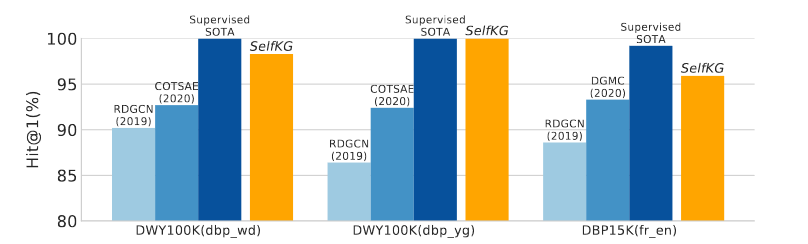
\includegraphics[width=\textwidth]{figure/hit@1.png}
  \caption{Hit@1 on DWY100K and DBP15K for SelfKG (0\% of training labels) and SOTA supervised (100\% of training labels) entity alignment. Without using any labels, the self-supervised SelfKG outperforms most of supervised models.}
  \Description{}
  \label{fig:teaser}
\end{teaserfigure}


%%
%% This command processes the author and affiliation and title
%% information and builds the first part of the formatted document.
\maketitle
%%=================================================================================
\section{Introduction}

In recent years, the rapid growth of the Internet has led to the creation of an increasing number of large-scale Knowledge Graphs (KGs) \cite{hogan2021knowledge} containing complementary information in various domains. Meanwhile, with the development of the initiative, the amount of semantic data on the Web is increasing, and one of the main challenges for various application domains is to integrate more and more independently designed entities that exist in different Knowledge Graphs, so that large-scale Knowledge Graphs can be efficiently coordinated with each other. Therefore, how to discover links between different knowledge graph instances becomes an important problem to be solved in various fields

Especially, with the rapid development of knowledge graphs in recent years, a large number of knowledge graphs have emerged \cite{hogan2021knowledge}. However, many knowledge graphs are currently constructed by different organizations and individuals, which have specific needs and are not uniform in design and construction, and thus have heterogeneity and redundancy problems with each other. Knowledge fusion aims to align and merge the information such as heterogeneity and redundancy in knowledge graphs to form a global unified knowledge identity and association.

Entity Alignment (EA)  \cite{liu2020exploring,zhao2020experimental}is the crucial technique of knowledge graph fusion process, and the main purpose is to discover equivalent entities between different knowledge graphs. As the knowledge contents of different knowledge graphs have different sources and different human understanding, the textual expressions referring to the same thing will be diverse. This is a significant problem of fusion and integration of different knowledge graphs, which affects the fulfillment of shared data. Therefore, the research on knowledge fusion based on knowledge graphs is significant for the subsequent technical exploration and development of big data integration and harmonization.

In this paper, we will present the relevant studies and commonly used models of entity alignment and analyze their advantages. Based on this, an attempt is made to analyze the rationale for the outstanding performance of $SelfKG$ models (in semi-supervised/unsupervised groups). And experiments are designed to verify the outstanding performance performance of Self-KGs, using previous models as a comparison.

\textbf{Contributions. } 

In this paper, Li selected and detailed the datasets $DWY100K_{dbp\_wd}$ and $DBP15K$ to be used in the task. the data was cleaned in the code using feature engineering, which contributed to the construction and Self-KGs previously used for comparison models. finally responsible for presenting the baseline and comparison results.

$Lin$ presents the technical background of entity alignment and reviews previous entity alignment methods, including those based on similarity calculation and relational reasoning. The strengths and weaknesses between the different methods are also analyzed in depth, which helps to analyze how the$ Self-KGs$ model can achieve such an outstanding performance in the semi-supervised case. Several previous models are reproduced with the help of Li for study and comparison.

$Hunag$ details how the advantages of the previous work are summarized in Self-KGs, explaining the key models and formulations that play a role. The main part of the $Self-KGs$ model is reproduced in the project, and the hyperparameters of the model are tuned and the results are calibrated and plotted.

In addition, special thanks to $Colab$ provided by Google, the models for this experiment are all run on the $Colad$ platform.

In this paper, We review the traditional entity alignment approach. The models and formulas, which play a key role in the reproduction of Self-KGs, are presented in detail. For the traditional methods, entity alignment methods based on similarity calculation and relational reasoning are categorically introduced, and the utilization of character features, attribute features, and relational features by each type of methods is studied in depth, while the advantages and shortcomings between different methods are analyzed in depth.

For entity alignment methods based on knowledge representation learning, this paper focuses on the discussion, analysis and comparison of. This paper unifies the three modules—alignment, interaction, and embedding—that make up the class of entity alignment techniques into a single framework and elaborates each method based on those three components. Existing methods are grouped into eight classes based on structure information, attribute information, entity name information, entity description information, comprehensive information, etc., according to the various types of knowledge map information used by the methods. Each of the eight categories of approaches is presented and thoroughly examined. On the basis of knowledge representation learning, an additional comprehensive comparison analysis of entity alignment techniques is conducted. The findings of the analysis demonstrate that the use of many pieces of information and scientifically sound iterative approaches can enhance the performance of the procedures.

In addition, the use of traditional models as reference targets reflects the advancement of Self-KGs

\section{Traditional Entity Alignment Method}

 Most of the traditional entity alignment methods have focused on syntax and structure, especially the early entity alignment and mapping techniques focused mainly on computing the distance of labels and characters between entities. The traditional entity alignment methods address the entity alignment problem from two main perspectives: one is based on similarity computation to compare symbolic features of entities \cite{cohen2002learning} and the other is based on relational reasoning \cite{halpin2010owl}, and recent studies also use statistical machine learning to improve accuracy.

This section provides a detailed overview of the existing traditional entity alignment methods, as well as an in-depth study of the utilization of character features, attribute features, and relationship features for each type of method, and a comparative analysis.


\subsection{Entity alignment method Based on Similarity Calculation}

Methods based on similarity computation for entity alignment using Term-Frequency InverseDocumentFrequency (TFIDF) \cite{cohen2002learning} , active learning and machine learning classifiers and NGram matching/edit distance/number matching \cite{sarawagi2002interactive}, synonym set and semantic verification \cite{jean2009ontology}, and filtering machines \cite{arasu2010active} compute the similarity between entities. Actually, it is the addition of machine learning classifiers \cite{sarawagi2002interactive}, active learning \cite{sarawagi2002interactive}, semantic verification \cite{jean2009ontology}, and filter blocking \cite{arasu2010active} to the similarity computation to improve the performance of the entity alignment algorithm.

\subsubsection{TFIDF-based Entity Alignment Method}

TFIDF is a common weighting technique used in information retrieval and text mining. TFIDF is a statistical method for evaluating the importance of a word for a collection of documents or one of the documents in a corpus. The importance of a word increases proportionally with its number of occurrences in a document, but decreases inversely with its frequency in a corpus. In a given document, term frequency (TF) refers to how often a given word appears in that document. This number is normalized to the number of words (term count) to prevent it from biasing towards longer documents. $TF_i$ represents the number of times a word is The number of occurrences, usually normalized.

\begin{equation}
{\mathrm  {TF_{{i,j}}}}={\frac  {n_{{i,j}}}{\sum _{k}n_{{k,j}}}}
\end{equation}
The above equation assumes that there are k words in the file $d_{{j}}$, $n_{k,j}$ is the number of times $t_{k}$ appears in the file $d_{j}$ is the number of times $t_{k}$ appears in the file $d_{j}$

The inverse document frequency (IDF) is a measure of the general importance of a word. The IDF of a particular term can be obtained by dividing the total number of documents by the number of documents containing the term, and taking the quotient as a logarithm of 10.The key concept of IDF is that if there are fewer entries containing a word, the greater the value of IDF if the word has good entry differentiation.

\begin{equation}
      {IDF_{i}} =\lg {\frac {|D|}{|\{j:t_{i}\in d_{j}\}|}}
\end{equation}
Among them :

\begin{itemize}
    \item |D|: Total number of documents in the corpus
    \item $|\{j:t_{{i}}\in d_{{j}}\}|$: number of files containing the word $t_{{i}}$ (i.e., the number of files with $n_{{i,j}}\neq 0$) If the word is not in the profile, it results in a zero denominator, so in general use 
\end{itemize}
Then we can get the formula of TFIDF:

\begin{equation}
    {\mathrm  {TF{}IDF_{{i,j}}}}={\mathrm  {TF_{{i,j}}}}\times {\mathrm  {IDF_{{i}}}}
\end{equation}

Cohen \cite{cohen2002learning} used TFIDF to calculate the distance between entity names
and the distance is in the threshold range to indicate a match between the two. By traversing
through all entity pairs $E_1 \times E_2$ to obtain the set of candidate entity pairs and train the two The classification function is trained to perform entity alignment. 

The aim of the algorithm is to acquire a set of matched entity pairs. {$y=\left\{\left(e_{1}, e_{1}^{\prime}\right),\left(e_{2}, e_{2}^{\prime}\right), \ldots,\left(e_{n}, e_{n}^{\prime}\right)\right\}$}, 
$e_1$ and $e_1^'$ are the entities in $E_1$ and $E_2$ and $y \subseteq E_{1} \times E_{2}$. {$y^{*}=\left\{\left(e_{1}^{*}, e_{1}^{\prime *}\right),\left(e_{2}^{*}, e_{2}^{\prime *}\right), \ldots\left(e_{n}^{*}, e_{n}^{*}\right)\right\}$ denotes a set of aligned sets of correct entity pairs, the loss function is defined as follows:

\begin{equation}
\begin{split}
    \text { Loss } \equiv\left|\left\{\left(e_{k}, e_{k}^{\prime}\right) \in y:\left(e_{k}, e_{k}^{\prime}\right) \notin y^{*}\right\}\right|\\+\left|\left\{\left(e_{k}^{*}, e_{k}^{\prime *}\right) \in y^{*}:\left(e_{k}^{*}, e_{k}^{\prime *}\right) \notin y\right\}\right|
\end{split}
\end{equation}

A high word frequency within a particular document, and a low document frequency of that word in the overall set of documents, yields a high-weighted $TFIDF$. Thus, the $TFIDF$ tends to filter out common words and retain important words.
However, the TFIDF is founded on the assumption that the words that are most meaningful for distinguishing documents should be those that occur with high frequency in the documents and less frequently in other documents in the entire document collection, therefore if the feature space coordinate system takes $TF$ word frequency as a measure, it can reflect the characteristics of similar texts. In addition, considering the ability of words to distinguish different categories, the $TFIDF$ method considers that the smaller the text frequency of a word's occurrence, the greater its ability to distinguish different categories of text. 

Therefore, the concept of inverse text frequency $IDF$ is introduced, and the product of $TF$ and $IDF$ is used as the taking measure of the feature space coordinate system, and it is used to complete the adjustment of the weights $TF$, and the purpose of adjusting the weights is to highlight the important words and suppress the minor words.But essentially $IDF$ is an attempt to suppress noise weighting and simply assumes that words with small text frequencies are more important and words with large text frequencies are more useless, which is obviously not entirely true. 

The simple structure of $IDF$ does not effectively reflect the importance of words and the distribution of feature words, making it unable to perform the function of adjusting weights well, hence the accuracy of the $TFIDF$ method is not very accurate.


\subsubsection{Machine Learning and Active Learning Based Entity Alignment Methods }

Sarawagi et al. \cite{sarawagi2002interactive}pointed out that in constructing entity alignment datasets when constructing entity alignment datasets, as manually discovering entity matches with comprehensive coverage using manual pairs is very difficult and the manual screening is time-consuming and laborious, limiting the algorithm scalability of the algorithm. He then proposed an active learning-based approach, which enables the system to interactively discover entity pairs that are difficult to be identified by the machine pairs that are difficult for machines to identify, thus improving the performance of the system.

In addition, Sarawagi et al. consider that the matching problem of entity pairs can be viewed as a classification problem, i.e., matching, non-matching, and fuzzy matching. Therefore, three classifiers were constructed for entity alignment using machine learning, namely, Decision Tree \cite{safavian1991survey}, Naive Bayesian \cite{wang2007naive}, and Support Vector Machine \cite{chang2001library}.
For the training of the three classifiers, a special discriminant mechanism is set up to speed up the training while improving the accuracy. Assuming that the classification results of the three classifiers agree, they are used as matched entity pairs; if there are differences in the results, such entity pairs are labeled using manual interaction.

Further, for large knowledge graphs, the size of entity pair $E_1 \times E_2$ may be out of control, and considering the scalability of the algorithm, Sarawagi \cite{sarawagi2002interactive} performed a simple filtering operation during the generation of the set of candidate matching entity pairs (i.e., matching operation when the initial letters of the entity pairs are the same) and reduce the size of the overall dataset by sampling the data. Also, the textual attributes of the entities (including NGram matching, overlapping word scores, and edit distance), numeric matching, and empty match padding techniques are further utilized in calculating the similarity of the generated candidate matching entities.

\subsubsection{Entity Alignment Methods Based on Synonym Sets and Semantic Verification}

Jean-Mary et al. \cite{jean2009ontology} proposed the Automated Semantic Matching of Ontology with Verification (ASMOV) algorithm, which uses additional synonym dictionaries on entity lexical features for similarity computation, while using semantic verification to further take entity semantics into account. For two entity pairs $(e,e^{\prime})$ in the knowledge graph, each entity contains label, ID and annotation information for lexical feature similarity $S_l$ computation, assuming that the additional lexicon set is $\Gamma$ and the synonym set is $syn(w)$, and the antonym set is $ant(w)$. The lexical feature similarity is calculated for $S_l$ as the formula:

\begin{equation}
    \begin{array}{l}
    S_{l}\left(e, e^{\prime}\right)= \\
    \left\{\begin{array}{l}
    1.0, \text { if } w=w^{\prime} \\
    0.99, \text { if } w^{\prime} \in \operatorname{syn}(w) \\
    0.0, \text { if } w^{\prime} \in \operatorname{ant}(w) \\
    \operatorname{Lin}\left(w, w^{\prime}\right), \text { if } w \in \Gamma \wedge w^{\prime} \wedge \Gamma \wedge w^{\prime} \notin \operatorname{syn}(w) \\
    \frac{\operatorname{tok}(w) \cap \operatorname{tok}\left(w^{\prime}\right)}{\max \left(|\operatorname{tok}(w)|,\left|\operatorname{tok}\left(w^{\prime}\right)\right|\right)}, \text { otherwise }
    \end{array}\right.
    \end{array}
\end{equation}

where $Lin(w,w^{\prime})$ represents the information similarity calculation method proposed by Lin et al. \cite{lin1998information}, $tok(w)$ represents the ordered strings in $w$, and $|tok(w)|$ denotes the number of ordered strings.
Furthermore, entity pairs larger than the similarity threshold need to be verified again by semantic verification to determine whether there is semantic contradiction, i.e., by formulating semantic rules such as multi-entity alignment, cross-alignment, disjoint assumption, etc., to further rigorously process the aligned entities to obtain more accurate aligned entities.

\subsubsection{Entity Alignment Methods Based on Filtering Mechanisms and Active Learning}

Arasu et al. \cite{arasu2010active} argue that previous active learning methods were unable to guarantee the quality of the datasets used for training and did not have a standard interface, resulting in a strong unpredictability of the results obtained. Secondly, the poor input scalability when traversing the entity set $E_1 \times E_2$ prevents the processing of large knowledge graphs.

They point out that the entity alignment problem can be simply viewed as a dichotomous classification problem, i.e., matching and non-matching. However, the main difference between entity alignment and classification problems is that the amount of non-matching data in the dataset far exceeds the amount of matching data. It is particularly important to balance the matching data with the non-matching data in the candidate matching entities. For this reason, an entity alignment method combining filtering mechanism and active learning is proposed.

Combining the dichotomous classification function $\mathcal{B}$ with the entity classification function $\mathcal{M}$  for end-to-end training, i.e., the input entity pairs are first filtered by the dichotomous classification function, and the passed entity pairs are then computed in detail. Combining the filtering mechanism with active learning can reduce the need for labeled data.

The filtering scheme uses a binary classification function as shown in Equation:

\begin{equation}
     \mathcal{B}: E_{1} \times E_{2} \rightarrow \text { true, false }
\end{equation}

For the knowledge graph entity alignment process only the entity pairs of $\mathcal{B}(e_1,e_2) = \text{true}$ are required for subsequent detailed calculations. When two candidate entities perform similarity calculation, $Jaccard$ distance is calculated using the attribute information of the entities

The $Jaccard$ distance calculation formula is as follows :
\begin{equation}
    \begin{array}{c}
         \mathcal{J}=\frac{\left|e_{1} \cap e_{2}\right|}{\left|e_{1} \cup e_{2}\right|} \# 
    \end{array}
\end{equation}

\begin{equation}
    \begin{array}{c}
         d_{\jmath}\left(e_{1}, e_{2}\right)=1-\mathcal{J}\left(e_{1}, e_{2}\right)
    \end{array}
\end{equation}

\subsection{Entity Alignment Methods Based on Relational Reasoning}

The entity alignment method based on relational reasoning mainly utilizes the relationships between entities in the knowledge graph by constructing probability functions \cite{suchanek2011paris} and relational similarity functions \cite{lacoste2013sigma} to reason about the semantic equivalence between relationships, and then realize the alignment between the entities corresponding to the relationships.

\subsubsection{Entity Alignment Method Based on Probability Functions}

Suchanek et al. \cite{suchanek2011paris} proposed the Probabilistic Alignment of Relations, Instances, and Schema (PARIS) algorithm, which probabilizes entity alignment by functionalizing relations and further performing probabilistic calculations based on the principles of relational reasoning, thus realizing the task of real body alignment.

To functionalize the relationship between entities, suppose the relationship between two entities is represented by a triple: $(e_1,r,e_2)$, then there exists the functional relationship $(x,r,y)$, and define $fun(x,r)$ as:
\begin{equation}
    \textit{fun}(r, x)=\frac{1}{|y: r(x, y)|}
\end{equation}

where $|y:r(x,y)|$ indicates the number of tail entities that satisfy the relation $r$ when the head entity $x$ is determined. 
Then, define the relational inverse function as :

\begin{equation}
    \textit{}{fun}^{-1}(r, x)=\textit{}{fun}\left(r^{-1}, x\right)
\end{equation}

Finally we can define the relational function :

\begin{equation}
    \textit{fun}(r)=\frac{|x: \exists y: r(x, y)|}{|x, y: r(x, y)|}
\end{equation}

Based on that, the relational inference formula in the following equation further probabilizes the entity matching, that is, calculates the probability that two entities may match, that is, to calculate the probability that two entities can match. 

\begin{equation}
    \begin{array}{c}
        \exists r, y, y^{\prime}: r(x, y) \wedge r\left(x^{\prime}, y^{\prime}\right) \wedge y \equiv \\
        y^{\prime} \wedge f u n^{-1}(r) \text { is high } \Rightarrow x \equiv x^{\prime}
    \end{array}
\end{equation}

Probabilizing the above inference formula yields the probability formula for the possible matching of entities as shown in the following equation $\textit{Pr}_{1}(x \equiv x^{\prime})$: 

\begin{equation}
    \begin{array}{l}
\textit{Pr}_{1}\left(x \equiv x^{\prime}\right):= \\
1-\prod_{r(x, y), r\left(x^{\prime}, y^{\prime}\right)}\left(1-f u n^{-1}(r)\right. \\
\left.\quad \times \textit{Pr}\left(y \equiv y^{\prime}\right)\right)
\end{array}
\end{equation}

Where probability $Pr_1$ represents the probability that two entities may match. Since the same mismatch exists in the actual reasoning process, it is necessary to further define the probability $Pr_2$ that two entities do not match, and the corresponding relational reasoning formula is shown below : 

\begin{equation}
    \begin{array}{c}
\exists r, y:(x, y) \wedge\left(\forall y^{\prime}: r\left(x^{\prime}, y^{\prime}\right) \wedge f u n(r)\right. \text { is high } \\
\left.\Rightarrow y \not \equiv y^{\prime}\right) \Rightarrow x \not \equiv x^{\prime}
\end{array}
\end{equation}

Probabilizing the above inference formula yields a probability formula for two entities that do not match

\begin{equation}
    \begin{array}{l} 
        \textit{Pr}_{2}\left(x \equiv x^{\prime}\right):= \\
        \prod_{r(x, y)}\left(1-\textit{fun}(r) \prod_{r\left(x^{\prime}, y^{\prime}\right)}(1\right. \\
        \left.\left.-\textit{Pr}\left(y \equiv y^{\prime}\right)\right)\right)
    \end{array}
\end{equation}

Finally, the two probability formulas are combined to obtain the final entity alignment probability $Pr_3$. The final probability value $Pr_3$ is used to determine whether the two entities are aligned or not.

\subsubsection{Entity Alignment Method Based on Relational Similarity Function}

Lacoste et al. \cite{lacoste2013sigma} proposed the Simple Greedy Matching for Aligning Large-Knowledge Bases (SiGMa) algorithm, which uses the greedy idea to perform a local search using the string, attribute and structure information of entities to complete the entity alignment between different knowledge maps.

The entity alignment process is divided into two main parts :
\begin{itemize}
    \item Constructing a similarity function based on attribute information.
    \item Build an adjacency graph using the matched entity pairs to construct the adjacency graph.
\end{itemize}

The $SiGMa$ algorithm utilizes the attribute information and relationship information of the entities to compute the attribute triples and relationship triples to obtain the aligned entities.

Suppose that for two knowledge graphs the set of entities $E_1 \times E_2$ is represented by the matrix $y$, and  $y_{i j}=(i, j): i \in E_{1}, j \in E_{2}$.If two entities $i$ and $j$ are matching entities, then $y_{ij}=1$, otherwise $y_{ij}=0$.Entity similarity $S_{ij}$ and relationship similarity $G_{ij}$ need to be calculated in the entity matching process.Construct the entity matching objective function $Obj(y)$ as follows :

\begin{equation}
    \begin{array}{l}
    \sum_{(i, j) \in E_{1} \times E_{2}} y_{i j}\left[(1-\alpha) S_{i j}+\alpha G_{i j}(y)\right] \\
    \textit { where } G_{i j} \doteq \sum_{(k, l) \in \mathcal{N}_{i j}} y_{k l} w_{i j, k l}
    \end{array}
\end{equation}

in which $\alpha$  is a balancing parameter between entity similarity and relationship similarity and is set to $0.25$ in the experiment. $N_{ij}$ indicates the set of local neighboring entities of entities $i$ and $j$. $W_{ij,kl}$ denotes the case where entities $k$ and $l$ are known to match, and is the weight parameter for calculating the relational similarity $G_{ij}$. The weights need to be determined according to the degree of contribution of neighboring entities $W_{ij,kl}$. The calculation formula is as follows : 

\begin{equation}
    \begin{array}{l}
    \gamma_{i} \doteq \frac{1}{2}\left(1+\sum_{k \in \mathcal{N}_{i}} w_{i k}\right)^{-1} \\
    \gamma_{j} \doteq \frac{1}{2}\left(1+\sum_{l \in \mathcal{N}_{j}} w_{j l}\right)^{-1}
    \end{array}
\end{equation}

The calculation of the similarity $S_{ij}$ of entities is divided into two parts: entity and attribute string similarity $String(i,j)$ and attribute set similarity $Prob(i,j)$, as follow :

\begin{equation}
    S_{ij} = (1-\beta)\textit{String(i,j)} + \beta \textit{Prob(i,j)}
\end{equation}

where $\beta$ is the equilibrium parameter, which is set to 0.25 in the experiment. Suppose entity $e_1$ contains attribute $p_1,p_2,\cdots,p_n$ and the attribute value is $v_1,v_2,\cdots,v_n$, entity $e_2$ contains attribute $q_1,q_2,\cdots,q_n$ and the attribute value is $l_1,l_2,\cdots,l_n$. The string similarity $String(i,j)$ and attribute set similarity $Prob(i,j)$ are calculated as follows :

\begin{equation}
    \begin{array}{l}
    \operatorname{string}(i, j) \\
    =\frac{\sum_{v \in\left(w_{i} \cap w_{j}\right)}\left(w_{v}^{1}+w_{v}^{2}\right)}{\operatorname{smoothing}+\sum_{v \in \mathcal{W}_{i}} w_{v}^{1}+\sum_{v^{\prime} \in \mathcal{W}_{j}} w_{v^{\prime}}^{2}} \\
    \end{array}
\end{equation}
and
\begin{equation}
    \begin{array}{l}
    \operatorname{prob}(i, j) \\
    =\frac{\sum_{(a, b) \in M_{12}}\left(w_{p_{a}, v_{a}}^{1}+w_{q_{b}, l_{b}}^{2}\right) \operatorname{Sim}_{p_{a}, q_{b}}\left(v_{a}, l_{b}\right)}{2+\sum_{a=1}^{n_{1}} w_{p_{a}, v_{a}}^{1}+\sum_{b=1}^{n_{2}} w_{q_{b}, l_{b}}^{2}}
    \end{array}
\end{equation}

where $W_i$ denotes the set of words in entity $i$, $W_i^1$ denotes the inverse document frequency IDF (See the previous chapters) of word $v$ in the set of entities $E_1$, $Smoothing$ is a smoothing term added to the denominator to make the long string contain as many co-occurring short words as possible. $M_{12}$ represents the set of aligned attributes, $W_{p_a,p_a}^1$ indicates the IDF of the attribute value of entity $e_1$, $W_{q_b,l_b}^1$ indicates the IDF of the attribute value of entity $e_2$. $Sim_{p_a,v_a}(v_a,l_b)$ is a $[0,1]$ function, 1 in case of $v_a=l_b$, otherwise 0.




\subsection{Comparative Analysis of Traditional Entity Alignment Methods }

As mentioned above, traditional entity alignment methods mainly focus on ontology alignment, and thus there is no uniform performance comparison for entity alignment tasks. The following table1 provides a comparative analysis of the traditional entity alignment methods. As can be seen from the above methods, it is difficult to give a unified similarity calculation function due to the various attributes of entities in the entity alignment process as well as the different domains involved. At the same time, this discrete attribute information ignores the semantic information implied in many aspects (such as the association semantics between attributes and the semantic information between triad structures, etc.)

\begin{table*}
\centering
\linespread{2}
\renewcommand\arraystretch{1.5}
\caption{Similarity-based calculation}
\label{tab:commands}
\begin{tabular}{c|c|c} 
\toprule
Author         & Constructed Entities                           & Feature Processing                                                         \\ 
\midrule
Cohen          & $E_1\times E_1$                                & TFIDF, string, prefix                                                      \\
Sarawagi       & $E_1\times E_1$, Initials and sample filtering & Machine learning and active learning                                       \\
Jean Jean-Mary & $E_1\times E_1$                                & Tags, IDs, annotations, synonym sets and semantic validation               \\
Arasu          & $E_1\times E_1$, Blocking function filtering   & Attribute set, machine learning,  active learning and filtering mechanism  \\
\bottomrule
\end{tabular}
\end{table*}

\begin{table*}
\centering
\linespread{2}
\renewcommand\arraystretch{1.5}
\caption{Relationship-based reasoning}
\label{tab:commands}
\begin{tabular}{c|c|c} 
\toprule
Author   & Constructed Entities                                                                                                                      & Feature Processing                                                                                               \\ 
\midrule
Suchanek & $E_1\times E_1$                                                                                                                           & Probabilization of relational equivalence reasoning                                                              \\
Sarawagi & \begin{tabular}[c]{@{}c@{}}Iterative pre-alignment of seed entities to neighboring entities,\\ Initials and sample filtering\end{tabular} & \begin{tabular}[c]{@{}c@{}}Constructing adjacency graphs based on \\relationships between entities\end{tabular}  \\
\bottomrule
\end{tabular}
\end{table*}


\begin{table*}
\centering
\caption{Advantages and disadvantages of various technologies}
\linespread{2}
\renewcommand\arraystretch{1.5}
\label{tab:commands}
\begin{tabular}{c|c|c} 
\toprule
Author         & Advantages                                                                                                                             & disadvantages                                                                                                                                                                        \\ 
\midrule
Cohen          & Low complexity and easy to calculate                                                                                                   & Poor input scalability                                                                                                                                                               \\
Sarawagi       & \begin{tabular}[c]{@{}c@{}}Simple filtering of the input data set \\improves the processing of large-scale data\end{tabular}           & \begin{tabular}[c]{@{}c@{}}Manual annotation of seed entities: \\matching and non-matching.\end{tabular}                                                                              \\
Jean Jean-Mary & \begin{tabular}[c]{@{}c@{}}Multiple similarity calculations to improve\\ the accuracy of entity alignment.\end{tabular}                 & \begin{tabular}[c]{@{}c@{}}Complex calculations, relying on large amounts of \\additional information about entities, \\and poor performance for large data processing.\end{tabular}  \\
Arasu          & \begin{tabular}[c]{@{}c@{}}Integrated blocking and matching functions\\ to reduce the need \\for marker data and run faster\end{tabular} & \begin{tabular}[c]{@{}c@{}}Only the attribute information of the entity is considered,\\ no structure information is added.\end{tabular}                                              \\
Suchanek       & Align not only entities, but also relationships and classes                                                                            & Deal only with one-to-one relationships                                                                                                                                              \\
Lacoste        & \begin{tabular}[c]{@{}c@{}}The attribute information\\ and structure information of the entity are utilized.\end{tabular}               & \begin{tabular}[c]{@{}c@{}}Requires pre-alignment of entities, \\relationships and attributes, \\requiring extensive tagging of data.\end{tabular}                                      \\
\bottomrule
\end{tabular}
\end{table*}

\section{Representation learning Based Entity Alignment Method}

In the field of machine learning, feature learning or representation learning is a collection of techniques for learning a feature: transforming raw data into a form that can be efficiently exploited by machine learning. It avoids the hassle of manually extracting features and allows computers to learn to use features while learning how to extract them: learning how to learn.

The objective of representation learning is to use machine learning techniques to represent description objects as low-dimensional dense vectors, and the distance between two vectors reflects the semantic relationship between the two objects.

The application of representation learning to knowledge representation, Knowledge Representation Learning (KRL), aims to achieve a vector representation of entities and relationships between entities in the knowledge graph, by reducing high-dimensional entities and relationships to obtain a numerical representation of low-dimensional vectors.

Based on the ability of knowledge representation learning techniques to represent entities and relationships as low-dimensional vector spaces, many researchers have proposed entity alignment methods based on knowledge representation learning, and this class of approaches has become the main technique to solve the entity alignment problem nowadays.

This section follows with a focus, comparative analysis and summary of the entity alignment methods based on knowledge representation learning.
\subsection{Knowledge Representation Learning Technology}
The current mainstream knowledge representation learning techniques can be divided into three categories: translation models, semantic matching models, and deep models \cite{wang2017knowledge}.

\subsubsection{Translation Model}

Based on the $word2vec$ word vector model, Mikolov et al.\cite{mikolov2013distributed} found that the word vectors obtained from training can remain unchanged after a translation operation in the word vector space.

Researchers have proposed a variety of translation models inspired by this phenomenon. Representative translation models include $TransE$ \cite{bordes2013translating} and its extensions, which treat relationships as translations from head entities to tail entities.

In $TransE$  \cite{bordes2013translating} , for each triple $(h,r,t)$, the relations are considered as connections of head and tail entities, and the relations exist in the direction, and $TransE$ is also called the translation model.

However, $TransE$ still has a number of limitations, including :
\begin{itemize}
    \item Unable to handle complex relationships 1-N, N-1 and N-N. 
    \item $TransE$ learns each triplet in isolation, without considering multi-step relational paths, which contain much useful information.
\end{itemize}

To address these limitations, researchers have proposed a number of extensions to the $TransE$ \cite{chen2016multilingual} model. Among them, $MTrans$ targets different languages, $MTransE$ encodes entities and relations in separate spaces and allows cross-language transformation of arbitrary entity or relation vectors, and the embedding model of multilingual mapping retains the excellent properties when monolingual embedding is performed.

\subsubsection{Semantic Matching Model}
Semantic matching models mainly use similarity-based methods to infer relational facts, including DistMult \cite{yang2014embedding}, Complex Embeddings (ComplEx) \cite{trouillon2016complex}, Holographic Embeddings (HolE) \cite{nickel2016holographic}, etc.

$DistMult$ \cite{yang2014embedding} uses a relation-specific bilinear form to consider the connection between entities and relations, and the scoring function for the triple $(h,r,t)$ is given by the following equation :

\begin{equation}
    f_r(h,t)=h^TM_rt
\end{equation}

The relation $M_r$ is the matrix corresponding to the relation $r$. In order to reduce the number of relation parameters, $DistMult$ restricts $M_r$ to a diagonal matrix.

$HolE$ \cite{nickel2016holographic} employs a new idea: to represent entity pairs by the cyclic correlation of vectors, the cyclic correlation $ R_d \times R_d \rightarrow R_d $ is calculated as follows : 

\begin{equation}
    [a * b]_{k}=\sum_{i=0}^{d-1} a_{i} b_{(i+k) \bmod d}
\end{equation}

In addition, in $HolE$, the scoring function of the triad $(h,r,t)$ is given by the following equation:

\begin{equation}
    f_r(h,t) = sigmoid(r^T(h*t))
\end{equation}

\subsubsection{Deep learning models}

Deep models mainly focus on knowledge representation learning using deep learning techniques, including Projection Embedding (ProjE) \cite{shi2017proje}, Convolutional 2D Embeddings (ConvE) \cite{dettmers2018convolutional}, Relational Graph Convolutional Networks (R-GCN) \cite{schlichtkrull2018modeling}, etc.

$ProjE$, which uses a multilayer perceptron for modeling; $ConvE$, which uses convolutional and fully connected layers for modeling the connection of entities and relations; and $R-GCN$, which uses graph convolutional networks (GCNs) \cite{kipf2016semi}; $RSN$ \cite{guo2019learning}, which uses random wandering to select entities and learn the relational paths of the triples.

\subsection{Entity Alignment Methods Based on Knowledge Representation Learning}

Entity alignment methods based on knowledge representation learning have become the main technique for solving entity alignment problems with good results, and most of them use translation models or GraphNeuralNetwork (GNN) for knowledge representation learning because of their strong robustness and generalization ability.

\subsubsection{Entity Alignment Using Structural Information}

This type of entity alignment method performs entity alignment with the help of knowledge graph structural information. Specifically, the structural information includes as follows :
\begin{itemize}
    \item The relational triples in the knowledge graph in the format $(E,R,E)$, e.g. $(Japan, Capital, Tokyo)$.
    \item Relationship paths.
    \item Neighborhood information.
\end{itemize}

Remarkably, structural information is extremely valuable for entity alignment tasks. The vast majority of current entity alignment methods make use of structural information. However, alignment may be more limited when there is insufficient structural information in the knowledge graph.

There is a class of methods that use relational triples as structural information, and this class of methods captures structural features in relational triples using the knowledge representation learning methods are usually translation models, and many methods in use this strategy when utilizing structural information.

$MTransE$ \cite{chen2016multilingual} proposed a cross-linguistic knowledge graph embedding model, which consists of two main parts

\begin{itemize}
    \item The entities and relations of the two knowledge graphs are embedded separately based on the relational triad using the TransE model, and the embedding spaces of the two knowledge graphs are independent of each other.
    \item The transformation method between the embedding space of two knowledge graphs is constructed with the following loss function formula.
\end{itemize}

\begin{equation}
    L=\sum_{\left(T, T^{\prime}\right) \in \delta\left(G_{1}, G_{2}\right)} S_{a}\left(T, T^{\prime}\right)
\end{equation}

Where $G1$ and $G2$ represent the knowledge graphs of two different languages, $\delta\left(G_{1}, G_{2}\right)$ represents the set consisting of the already aligned triad pairs in the two knowledge graphs, and $S_{a}\left(T, T^{\prime}\right)$ is the method to score the already aligned triad pairs.

The model proposes three methods of scoring, the first is distance-based axis calibration, which scores two triads according to their distance from each other; the second is translation vector, which means that the alignment across the knowledge map is also considered as a relationship, and this relationship is also considered as the process of translation; the third is linear transformation, which means that the transfer matrix is defined and the two aligned triads are transformed between each other by the transfer matrix. Finally, entity alignment is then performed according to the embedding of the knowledge map, and the experimental results show that the linear transformation works best.

In addition, there are also methods that use relational paths as structural information, which capture structural features in relational paths, using knowledge representation learning methods that are usually also translation models and methods that use adjacency information as structural information This class of methods assumes that entities that express the same meaning in different knowledge graphs have similar adjacency information, and most of these methods use graph neural networks (GNN) \cite{scarselli2008graph} for embedding.

\subsubsection{Entity Alignment Using Attribute Information}

The above approaches use the structural information in knowledge graphs and have some limitations on the patterns and structures of different knowledge graphs. However, a large number of heterogeneous knowledge graphs exist in the real world. Therefore, a schema-independent entity alignment approach (Schema-Agnostic) is proposed in the literature \cite{teong2020schema}.

Considering entity alignment as a classification problem, labels (matching or non-matching) of candidate entity pairs are generated. The attribute values of the entities are concatenated and trained using Bidirectional Encoder Representations from Transformers (BERT) \cite{devlin2018bert}.

\subsubsection{Entity Alignment Using Structural and Attribute Information}

The methods in the above two sections utilize the structural and attribute information of the knowledge graph for representation learning, respectively. When only structural information is utilized, the attribute information of the knowledge graph is ignored, while the attribute information has the feature of higher accuracy and can enhance the entity alignment effect.

However, using only attribute information again ignores the structure of the knowledge graph and the connection between entities. For this reason, some approaches propose to use a combination of structural and attribute information for entity alignment.

Specifically, attribute information refers to attribute triples in the knowledge graph in the format of $(E,A,V)$, e.g. $(Homo, age, 24)$. Some entity alignment methods introduce attribute information to complement the structural information, which are mainly classified into the following two types.

\begin{itemize}
    \item Using structural information and names of attributes.
    \item Introduce the specific value of the attribute.
\end{itemize}

The attribute relevance embedding considers the correlation between attributes, and multiple attributes are considered relevant if they are often used together to describe an entity. For example, longitude and latitude are related because they are often combined to form coordinates that are used to describe a location.

$JAPE$ \cite{sun2017cross} assumes that similar entities have similar related attributes, and the algorithm consists of two modules, Structure Embedding (SE) obtained from relationship triples and Attribute Embedding (AE) obtained from attribute triples, and finally combining $SE$ and $AE$ to obtain the embeddings of all entities in the two knowledge graphs.

$CTEA$ (Context and Topic Enhanced Entity Alignment) framework also utilizes structural information and attribute names. $CTEA$ generates candidate sets for each source entity based on the attribute information of the entity, generates entity structural embedding and entity context representation based on the structural information of the entity, calculates the corresponding similarity matrix based on the entity structural embedding and context representation respectively, and weighted sums the two similarity matrices to obtain the final similarity matrix. Then the alignment result is found in the corresponding candidate set.

In addition, several methods further introduce specific values for attributes based on the use of structural information and attribute names.

The Self-learning and Embedding based method for Entity Alignment (SEEA) \cite{guan2019self} algorithm views entity alignment as a special kind of cross-network relationship and there is only this one relationship type in this algorithm. The algorithm embeds entities, attributes and attribute values based on the relationship triad and attribute triad, and also introduces a weighting mechanism for attributes, where important attributes will have higher weights, after which entity alignment is performed through an iterative mechanism, and the embedding is updated iteratively based on the results of the algorithm alignment.

\subsubsection{Entity Alignment using Structure Information and Entity Name Information}

Currently, most entity alignment methods infer from structural and attribute information, but most entities in real-world knowledge graphs contain often limited structural and attribute information. For this reason, some approaches propose to further use entity name information for entity alignment.

The Degree-Aware Entity Alignment In Tail (DAT) \cite{zeng2020degree} model uses Recurrent Skipping Networks (RSNs) \cite{guo2019learning} knowledge representation model for structural embedding, and the entity names are embedded at the character level by calculating the structural similarity and entity name similarity of two entities and combining them according to their weights using an attention mechanism .

The Collective Entity Alignment (CEA) \cite{zeng2020collective} model uses $GCN$ for structural information embedding and averages the entity name word vectors for embedding.

\subsubsection{Entity Alignment using Structure Information, Attribute Information and Entity Description Information}

The Hybrid Multi-Aspect Alignment Network (HMAN) \cite{yang2019aligning} model proposes to use a combination of multifaceted information for entity alignment, such as: entity labels, topological information, relationship types, attributes and text descriptions. The multifaceted information is added while embedding structural information using $GCN$, and the three aspects of topological information, relations and attributes are used as input to $GCN$ at the same time, instead of just as external auxiliary information. 

Finally, the text description information is learned using BERT embedding, which combines structural embedding and text description information embedding for integrated entity alignment. The multilayer $GCN$ is used to obtain the topological information of the knowledge graph, and the fully connected layer and high-speed gate mechanism are used to perform the relationship and attribute embedding, and finally the topological information, relationship information and attribute information are connected.

In addition, Multi-view KG Embedding (MultiKE) \cite{zhang2019multi} framework, utilizes both structural information, attribute information and entity name information. For entity names, each word in them is first embedded separately, and in order to capture the semantic information of words in different expressions, word embeddings are used if the words have word embeddings, otherwise the average of character embeddings is used as embeddings, and finally all word embeddings are concatenated and then compressed into one name embedding in an unsupervised manner. 

For the relationships between entities, the framework uses $TransE$ to get the relationship embeddings. For attributes of entities, the framework uses Convolutional Neural Networks (CNN) to capture the information in attributes and their values, and first connects the attribute name embeddings and attribute value embeddings horizontally and then feeds them into CNN to get the compressed attribute embeddings.

In considering the combination of these three embeddings to generate the embeddings of entities, the framework proposes three strategies. The first one is to combine based on a weighting mechanism, where the three embeddings are weighted and summed as the embedding of the entity. The second one is to combine based on shared space, mapping the space of each embedding into the same space by an orthogonal mapping matrix. The third one is to train all embeddings jointly during training, so that the consistency between the entity embeddings in the same embedding space and the three embeddings is as large as possible.

In addition, to better learn the connection between two knowledge graphs, the framework proposes two methods of reasoning across knowledge graphs based on aligned entities, relationships and attributes to generate more triples.

\subsubsection{Entity Alignment using Structure Information, Attribute Information, Entity Name Information and Entity Description Information}

BERT-based INTeraction model (BERT-INT) \cite{tang2020bert} is an embedded representation of entities using entity name and entity description information as input to train entities, and similarity is calculated using adjacency information, relationship and attribute information between entities.

The $BERT-INT$ model first uses $BERT$ as the basic representation unit to embed names/descriptions, attributes and values of entities, and models the neighbor view and attribute view interactions to compute the interactions between these embeddings.

Suppose two entity sets $E^\prime$ and $E^\prime$ are from different knowledge graphs, where ${r_1,\cdots,r_n}$ and ${e_1,\cdots,e_n}$ represent the relationship between the entity set $E$ and the entity, ${r_1^\prime,\cdots,r_n^\prime}$ and ${e_1^\prime,\cdots,e_n^\prime}$ represent the relationship between the entity set $E^\prime$ and the entity

${a_1,\cdots,a_n}$  and ${v_1,\cdots,v_n}$  represent the attributes and attribute values of the entity set $E$, and ${a_1^\prime,\cdots,a_n^\prime}$ and ${e_1^\prime,\cdots,e_n^\prime}$ represent the attributes and attribute values of the entity set $E^\prime$.

In the attribute information interaction module, the attributes and attribute values of the candidate entity pairs, $C(a_i)$ and $C(v_i)$. The relationships and entities, $C(a_i)$ and $C(v_i)$, need to be entered in the adjacency information interaction module.

Finally, the $BERT$ based interaction module combines entity adjacency information, neighboring entity relationships and attribute information to calculate entity similarity synthetically to complete entity alignment.

\subsection{Relevant Model Comparison and Analysis}

\begin{table*}
\centering
\linespread{2}
\renewcommand\arraystretch{1.5}
\caption{Comparison of Various Models}
\label{tab:commands}
  \label{tab:commands}
  \begin{tabular}{c|c|c|c|c}
    \toprule
    & \multicolumn{4}{c}{Information Type} \\
    Model & Structure  & Attribute & Entity name & Entity description\\
    \midrule
    $MTransE$\cite{chen2016multilingual} & \checkmark & \XSolid  & \XSolid  & \XSolid   \\
    $MuGNN$\cite{cao2019multi} & \checkmark & \XSolid  & \XSolid  & \XSolid  \\
    $TransEdge$\cite{sun2019transedge} & \checkmark & \XSolid  & \XSolid  & \XSolid  \\
    $KECG$\cite{li2019semi} & \checkmark & \XSolid  & \XSolid  & \XSolid  \\
    $AliNet$ \cite{sun2020knowledge} & \checkmark & \XSolid  & \XSolid  & \XSolid  \\
    $SelfAttention-GCN$\cite{chen2020learning} & \checkmark & \XSolid  & \XSolid  & \XSolid  \\
    $JAPE$ \cite{sun2017cross}& \checkmark & \checkmark & \XSolid  & \XSolid  \\
    $SEEA$ \cite{guan2019self}& \checkmark & \checkmark & \XSolid  & \XSolid  \\
    $HGCN$\cite{wu2019jointly} & \checkmark & \XSolid  & \checkmark & \XSolid  \\
    $DRGCN$\cite{wu2019relation} & \checkmark & \XSolid  & \checkmark & \XSolid  \\
    $DGMC$\cite{fey2020deep} & \checkmark & \XSolid  & \checkmark & \XSolid  \\
    $DAT$\cite{zeng2020degree} & \checkmark & \XSolid  & \checkmark & \XSolid  \\
    $MultiKE$ \cite{zhang2019multi}& \checkmark & \checkmark & \checkmark & \XSolid  \\
    $BERT-INT$\cite{tang2020bert} & \XSolid  & \checkmark & \checkmark & \checkmark \\
    \bottomrule
  \end{tabular}
\end{table*}

According to the different information utilized, the entity alignment methods based on knowledge representation learning are classified into three categories: utilizing only structural information, utilizing structural information and additional information (attribute information, entity name information, entity description information, etc.), and utilizing only additional information.

According to the different embedding methods, it is further subdivided into three categories based on $TransE$ and $GCN$ .

\subsubsection{Using Only Structural Information}

Based on the utilization of $TransE$ structural information, $TransEdge$ \cite{sun2019transedge} obtains the best results, indicating that the embedding representation of the knowledge graph should be done not only with vector embedding of head and tail entities, but adding the embedding of relationships between entities can better represent the knowledge graph. Both $TransEdge$ \cite{sun2019transedge}  and $KECG$ \cite{li2019semi}  consider the relationships between entities, and among them $KECG$ \cite{li2019semi} , which uses $GAT$ to label the relationship weights, obtains the worst experimental results.

Based on the utilization of $GCN$ structural information, $AliNet$ \cite{sun2020knowledge} adopts the strategy of considering multi-hop entities differently but treating directly neighboring entities uniformly.

Based on the utilization of $GNN$ structural information, $MuGNN$ \cite{cao2019multi} uses an attention mechanism to assign weights to the relationships between entities. In addition $MuGNN$ \cite{cao2019multi} requires not only pre-alignment of aligning entities, but also aligning relationships, which is in labeling the training data time-consuming and labor-intensive.

From the above analysis, it can be seen that the entity alignment method using only structural information, the $TransE$ based embedding method performs poorly on the whole. The main reason is that the use of $TransE$ to construct relational triples lacks consideration of the overall structural information of the knowledge graph, thus losing some structural information. In addition, it can be seen from the method which is based on GCN/GNN, compared to $MuGNN$ (2019) which obtained the best results in terms of experimental effectiveness in utilizing structural information. It indicates that the representation of embedding approaches based on $GCN$ or $GNN$ without any restrictions and constraints in representing entity and relation embeddings can lead to the transformed results destroying the similarity of structural information of the original knowledge graph and thus perform poorly on the entity alignment task.

\subsubsection{Using Structural and Additional Information}

 JAPE \cite{sun2017cross} adds a joint learning representation vector of attribute triples to the embedding representation, which co-embeds the structure of two KGs into a unified vector space and further refines the KGs by exploiting the attribute correlations in the KGs.

 The embedded method based on GCN. Both $RDGCN$ and $HGCN$ use additional information in the form of entity names, and both use pre-trained word vectors of entity names in their initialization. $RDGCN$ uses an attention mechanism, but assigns weights to the relationships between all neighboring entities, which leads to error propagation and therefore performs poorly.

 Both $RDGCN$ and $HGCN$ represent embeddings of relationships between entities, and both use a high-speed gate mechanism to mitigate error propagation in GCN, while $HGCN$ uses a bootstrap training strategy, making $HGCN$ slightly more effective than $RDGCN$.

 GCN performs slightly better than $TransE$ in terms of considering structural and attribute information

\subsubsection{Use Only Additional Information}

$BERT-INT$ \cite{tang2020bert} obtained a significant improvement in the overall results, showing that the semantic information of entities can be obtained very accurately with additional information beyond the experimental dataset.

This suggests that additional information is more conducive to entity alignment than structural information.

\section{SelfKG DEFINITION}
\begin{figure}[h]
    \centering
    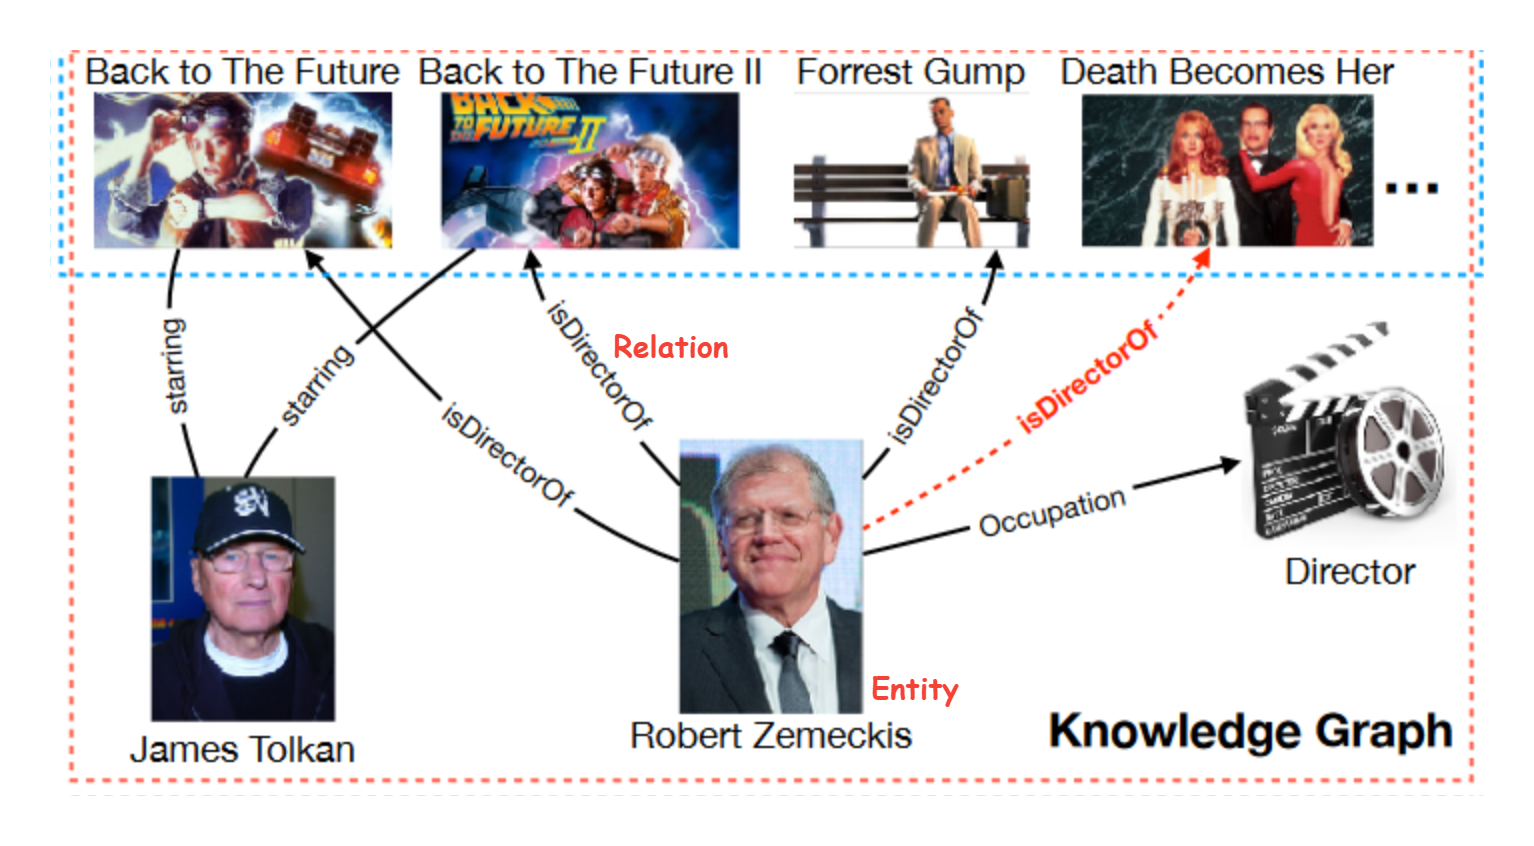
\includegraphics[width=1\linewidth]{figure/KG.png}
    \caption{Knowledge Graph\cite{10.1145/3308558.3313705}}
    \label{kg}
\end{figure}
Here let me describe the problem of entity alignment in Knowledge Graph. Conceptually, a Knowledge Graph can be represented as a set of triples $T$, each of which denotes the relation $r_{ij} \in R$ between two entities $x_i \in E$ and $x_j \in E$. In this work, we denote a Knowledge Graph as $G = {E, R, T}$ where $E, R$, and $T$ are its entity set, relation set, and triple set, respectively. Fig \ref{kg} shows what the Knowledge Graph is.

Given two Knowledge Graphs, $G_x = \{E_x , R_x , T_x\}$ and $G_y = \{E_y , R_y , T_y\}$, the set of the existing aligned entity pairs is defined as $S = \{(x, y)|x \in E_x , y \in E_y , x \Leftrightarrow  y\}$, where $\Leftrightarrow$ represents equivalence. The goal of entity alignment between $G_x$ and $G_y$ is to find the equivalent entity from Ex for each entity in $E_y$ , if existed.

Recently, a significant line of work has been focusing on embedding-based techniques for aligning entities in the vector space, e.g., training a neural encoder f to project each entity $x \in E$ into a latent space. Among these attempts, most of them focus on the (semi-) supervised setting in the sense that part of $S$ is used for training the alignment models \cite{chen2016multilingual,tang2020bert,wang2018cross,wu2019relation}. Due to the limited alignment labels across Knowledge Graphs in the real world, the paper instead proposes to study to what extent the entity alignment task can be solved in an unsupervised or self-supervised setting, under which none of the existing alignments in $S$ is available.
\subsection{Evaluation Metrics}
This section describes the most common metrics used to measure the performance of knowledge graph embedding models: HITS@1, HITS@10.

This metric is the average percentage of triads that rank less than n in the link prediction. The specific calculation is as follows:
\begin{gather}
    HITS@n=\frac{1}{\left | S \right |} \sum _{i=1}^{\left | S \right |}\mathbb{I}(rank_i\le n) 
\end{gather}
where $S$ is the set of triples and $\left | S \right |$ is the number of sets of triples. Besides, $\mathbb{I}(\cdot)$ is the indicator function (function value is 1 if the condition is true, otherwise it is 0). Generally, take n equal to 1, 3 or 10. the larger the indicator, the better.
\section{Methodlogy}
In this section, I will explain the role that supervision plays in entity alignment and then present the strategies that can help align entities without label supervision. To this end, I reviewed the SelfKG framework for self-supervised entity alignment across Knowledge Graphs carefully.
\subsection{The SelfKG Framework}
The main objective of SelfKG is to create a self-supervised objective that can direct its learning process in order to enable learning without labeling information. To do this, the paper suggests using the relative similarity metric between entities in two KGs (details illustrated in Section~\ref{3.2}). It introduces the self-negative sampling and multiple negative queues techniques to further enhance the self-supervised optimization of SelfKG. The initialization of entity embeddings in SelfKG, which is largely based on already-used methods like uni-space learning and GNN-based neighborhood aggregator, is then introduced.

The initialization of entity embeddings in SelfKG is largely built upon existing techniques, including the uni-space learning and GNN-based neighborhood aggregator.
\subsubsection{BERT}
\begin{figure}
    \centering
    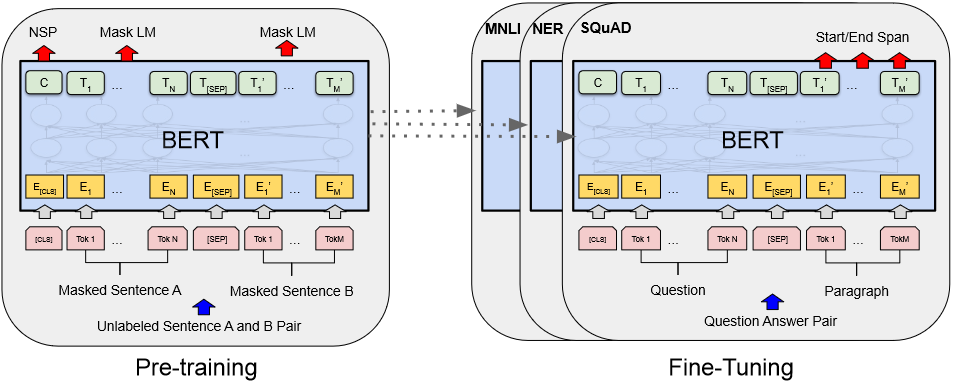
\includegraphics[width=1\linewidth]{figure/BERT.png}
    \caption{Overall pre-training and fine-tuning procedures for BERT\cite{devlin2018bert}}
    \label{bert}
\end{figure}
\cite{devlin2018bert}(Bidirectional Encoder Representations from Transformers) is a State-Of-The-Art language representation model developed by Google at that time. It was introduced in a paper published in 2018 by researchers at Google and it is shown in Fig \ref{bert}.

BERT is a transformer-based architecture that processes input text by masking some of the words and predicting the masked words given the context provided by the other words in the sentence. This process, called "masked language modeling," allows BERT to learn contextual relationships between words (i.e., semantics) and how they are used in different sentences.

One of the key features of BERT is that it is a bidirectional model, which means that it takes into account the context before and after each word in the input text. This is in contrast to traditional language models, which process text only in one direction (e.g., left to right or right to left). The bi-directionality of BERT allows it to better capture the context of a word, which is important for many natural language processing tasks such as language translation, text classification, and question answering.

BERT has been widely adopted and has achieved state-of-the-art results on a variety of natural language processing tasks. It has also inspired the development of many other transformer-based language representation models, such as RoBERTa, ALBERT, et al.
\subsubsection{Graph attention network}
\begin{figure}[h]
    \centering
    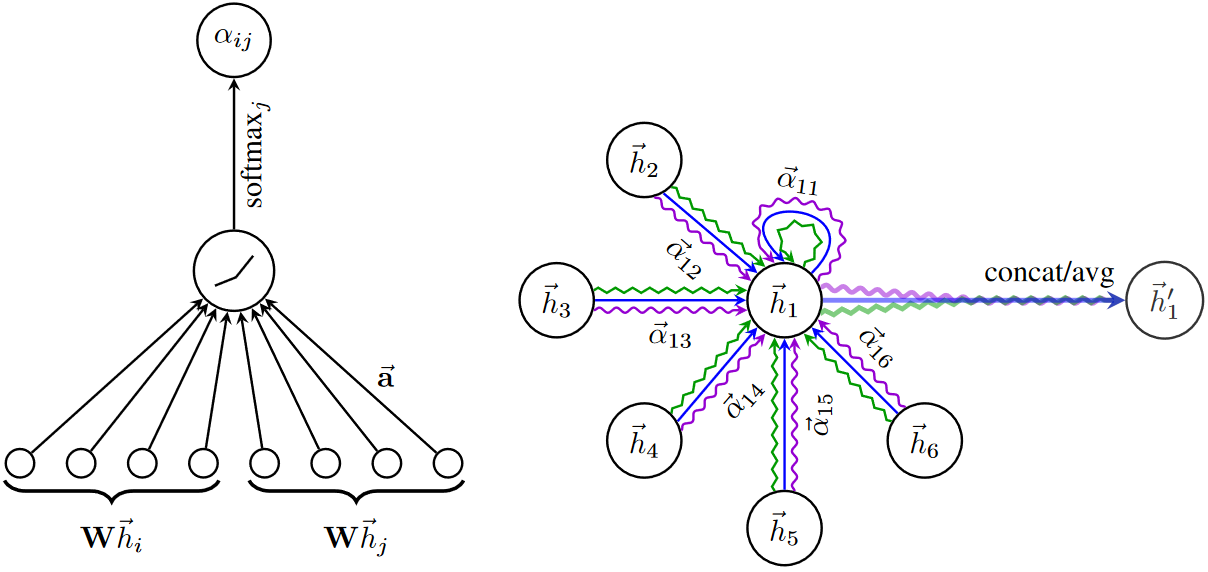
\includegraphics[width=1\linewidth]{figure/gat.png}
    \caption{Graph attention mechanism\cite{velivckovic2017graph}}
    \label{gat}
\end{figure}
A Graph Attention Network (GAT) is a type of neural network that operates on graph-structured data\cite{velivckovic2017graph}. It is particularly useful for learning representations of graph-structured data and for performing various types of prediction tasks on graphs, such as node classification and link prediction, which its mechanism is shown in Fig \ref{gat}.

GATs are based on the idea of self-attention, which is a mechanism used in natural language processing to allow a model to attend to different parts of the input text at different times. In the context of graph data, self-attention allows a GAT to weigh the importance of different nodes and edges in the graph when performing a prediction task. In this way, the attention mechanism can adapt to the specific characteristics of the graph and improve the model's performance.

A GAT consists of multiple "attention heads," each of which operates on a different part of the graph. Each attention head computes a weighted sum of the node representations in the graph, where the weights are learned using self-attention. The output of the attention heads is then combined and used to make a prediction.

GATs have been shown to be effective at learning rich representations of graph-structured data and have been applied to a wide range of tasks, including social network analysis\cite{kosaraju2019social}, recommendation systems\cite{wang2019kgat}, and protein-protein interaction prediction\cite{lai2022accurate}.

Here showing a common approach to implementing graph attention using self-attention. In this approach, let us represent each node in the graph as a feature vector, $h = \{\vec{h_1}, \vec{h_2},\dots, \vec{h_N} \},h_i \in \mathcal{R}^F$, where $N$ is the number of nodes, and $F$ is the number of features in each node. The layer produces a new set of node features (of potentially different cardinality $F^{'}$), $h^{'} =  \{\vec{h^{'}_{1}}, \vec{h^{'}_{2}},\dots, \vec{h^{'}_{N}}  \},  \vec{h^{'}_{i}} \in \mathcal{R}^{F^{'}}$ as its output. and we use self-attention to compute a weighted sum of these feature vectors. The self-attention weights are computed using the following equation:
\begin{align}
    e_{ij} = A(W\vec{h_i},W\vec{h_j})
\end{align}
First is a shared linear transformation, parametrized by a weight matrix, $W \in \mathcal{R}^{F^{'}\times F}$, and is applied to every node. then it performs self-attention on the nodes—a shared attention mechanism $A: \mathcal{R}^{F^{'}} \times \mathcal{R}^{F^{'}}\to \mathcal{R}$ computes attention coefficients. To make coefficients easily comparable across different nodes, we normalize them across all choices of j using the Softmax function:
\begin{align}
    \alpha _{ij} = Softmax(e_{ij})= \frac{exp(e_{ij})}{ \textstyle \sum_{k\in\mathcal{N}_i}exp(e_{ik})}
\end{align}
\subsubsection{Uni-space learning}
Recent (semi-) supervised entity alignment techniques have incorporated the concept of uni-space learning \cite{chen2016multilingual,tang2020bert,wang2018cross,wu2019relation}. The Paper demonstrates how they use it to support the self-supervised learning environment of SelfKG. Straightforwardly, the alignment task can be greatly aided by embedding entities from various Knowledge Graphs into a uni-space. With labeled entity pairs, it makes sense to use supervision to align various spaces into one. For example, aligned entities for training can be combined \cite{hao2016joint}, and entities from various embedding spaces can be projected into a uni-space using learning projection matrices with a lot of training labels \cite{chen2016multilingual,sun2017cross}. The problem is more difficult when it comes to multilingual datasets (like DBP15K). The availability of high-quality multi-lingual initial embeddings has been made possible by the pre-trained language models \cite{han2021pre}. For instance, recent research has utilized the multilingual BERT \cite{tang2020bert,zhang2019multi}. In SelfKG, we adopt LaBSE \cite{feng2020language}—a state-of-the-art multi-lingual pre-trained language model trained on 109 different languages—for embedding different knowledge graphs into a uni-space.
\subsubsection{Neighborhood aggregator}
To further improve the entity embeddings, the neighborhood aggregation is used to aggregate neighbor entities’ information to the center entity \cite{wang2018cross,xu2019cross}. In this work, authors directly use a single-head graph attention network \cite{velivckovic2017graph} with one layer to aggregate pre-trained embeddings of one-hop neighbors. Note that leveraging multi-hop graph structures has been recently explored for the problem of entity alignment. Though some studies \cite{fey2020deep,wang2018cross,wu2019relation} claim that they benefit from multi-hop neighbors, other works \cite{xu2019cross,zhang2018mego2vec} argue that one-hop neighbors provide enough information for most situations. In their ablation study, they found that the multi-hop information actually harmed the performance of Self-KG, which probably resulted from the distant neighbor noises that may be unignorable in a self-supervised setting. Therefore, to demonstrate the minimum requirement of self-supervision for entity alignment, they only involved one-hop neighbor entities during the aggregation.
\subsection{Relative Similarity Metric} \label{3.2}
The paper presents the self-supervised loss for entity alignment across Knowledge Graphs. First, it analyzes the supervised NCE loss for entity alignment. Then, it introduces the relative similarity metric for avoiding labeled pairs. Finally it derives the self-supervised NCE for SelfKG. In representation learning, the margin loss \cite{bordes2013translating,tang2020bert} and crossentropy loss \cite{zhang2019oag} have been widely adopted as the similarity metric. Without loss of generality, they can be expressed in the form of Noise Contrastive Estimation (NCE)\cite{gutmann2010noise}.

In the context of entity alignment, the NCE loss can be formalized as follows. Let $p_x, p_y$ be the distributions of two Knowledge Graphs $G_x, G_y$, and $p_{pos}$ denote the representation distribution of the positive entity pairs $(x, y) \in R_n times R_n$. Given a pair of aligned entities $(x, y) \sim p_{pos}$, negative samples $\{y^{-}_i\}_{i=1}^M \overset{i.i.d}{\sim}  p_y$, the temperature $\tau$ , and the encoder $f$ satisfies $\left \| f(\cdot) \right \|=1  $, we have the supervised NCE loss as:
\begin{gather}\label{3}
\mathcal{L}_{NCE}\overset{\bigtriangleup }{=}-log\frac{e^{f(x)^Tf(y)/\tau}}{e^{f(x)^Tf(y)/\tau}+\sum _ie^{f(x)^Tf(y_i^{-})/\tau}} \notag \\
=-\frac{1}{\tau}f(x)^Tf(y)+log(e^{f(x)^Tf(y)/\tau}+\sum_ie^{f(x)^Tf(y_i^{-})/\tau})   
\end{gather}
Here, the lefts side of the "$+$" is called "alignment" part and right side which in the $log$ is called "uniformity" part. The "alignment” term is to draw the positive pair close and the “uniformity” term is to push the negative pairs away. The paper illustrates how this NCE loss can be further adjusted for a self-supervised setting. An example of “pulling” and “pushing” entity pairs in Knowledge Graphs can be found in Fig \ref{rsm}. Previous studies have shown that the NCE loss has the following asymptotic properties:

\textbf{Theorem 1.} (Absolute similarity metric (ASM). For a fixed $\tau >0$ , as the number of negative samples $M \to \infty $, the (normalized) contrastive loss $\mathcal{L}_{NCE} (i.e., \mathcal{L}_{ASM})$ converges to its limit with an absolute deviation decaying in $O(M^{-\frac{2}{3}})$. If a perfectly-uniform encoder $f$ exists, it forms the exact minimizer of the uniformity term.

Theorem 1 makes the NCE loss an absolute similarity metric that requires supervision. However, note that despite potential ambiguity and heterogeneity for entities in KGs, the aligned pairs should share similar semantic meanings, if not exactly the name. Furthermore, the pre-trained word embeddings are known to capture this semantic similarity by projecting similar entities close in the embedding space, which can thus ensure a relatively large $f(x)^T f(y)$ in Eq. \ref{3}, i.e., the “alignment” term. 

Therefore, to optimize the NCE loss, the main task is then to optimize the “uniformity” term in Eq. \ref{3} rather than the “alignment” term. Considering the boundedness property of $f$, we can instantly draw an unsupervised upper bound of $\mathcal{L}_{ASM}$ by as follows.

\textbf{Proposition 1. Relative similarity metric (RSM).} For a fixed $\tau > 0$ and encoder $f$ satisfies $\left \| f(\cdot) \right \|=1  $, we always have the following relative similarity metric plus an absolute deviation controlled by a constant as an upper bound for $\mathcal{L}_{ASM}$:

\begin{gather}\label{eq2}
\mathcal{L}_{RSM}=-\frac{1}{\tau }+ \underset{\left \{y_i^{-}\right\}\overset{i.i.d}{\sim}p_y}{\mathbb{E}}\left[ log(e^{\frac{1}{\tau}+\sum_ie^{f(x)^Tf(y_i^{-})/\tau}}) \right] \notag\\
\le \mathcal{L}_{ASM} \le \mathcal{L}_{RSM} + \frac{1}{\tau}\left[ \underset{(x,y)\sim p_{pos}}{min}f(X)^Tf(y)  \right ]     
\end{gather}
By optimizing $\mathcal{L}_{RSM}$, the aligned entities are relatively drawn close by pushing non-aligned ones farther away. In other words, if we cannot draw the aligned entities close (e.g., no positive labels), we can instead push those not-aligned ones far away enough. By analyzing the commonly-used NCE loss for entity alignment, we find that the training can benefit more from pushing those randomly-sampled (negative) pairs far away than pulling aligned (positive) ones close. Thus, in SelfKG, we focus only on attempting to pushing the negatives far away such that we can get rid of the usage of positive data (i.e., labels).
\begin{figure}[h]
    \centering
    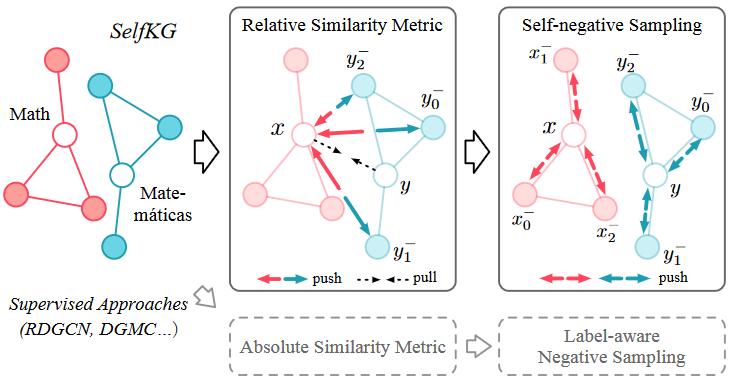
\includegraphics[width=1\linewidth]{figure/rsm.png}
    \caption{A conceptual comparison of SelfKG and supervised approaches. SelfKG employs the relative similarity metric (RSM) and self-negative sampling to avoid the use of supervision.}
    \label{rsm}
\end{figure}
\subsection{Self-Negative Sampling} \label{3.3}
In the analysis above, the paper demonstrates that to align entities without supervision, the focus of SelfKG is on sampling negative entity pairs—one from Knowledge Graph $G_x$ and the other from Knowledge Graph $G_y$ . During negative sampling, without supervision for label-aware negative sampling, it is likely that the underlyingly aligned entity pair is sampled as a negative one, i.e., collision happens. Normally, this collision probability can be ignored if a few negatives are sampled; but they discover that a large number of negative samples can be crucial to the success of SelfKG in Fig \ref{study}, under which the collision probability is non-negligible (Cf. Table 4), causing a performance drop by up to 7.7\%  
relatively. To mitigate the issue, the paper proposes to sample negatives $x_i^{-}$ from $G_x$ for entity $x \in G_x $, given that we are learning from the uni-space of $G_x and G_y$ . By doing so, we would avoid the conflict by simply excluding x, namely self-negative sampling.

However, there may be two other issues aroused consequently. First, due to the real-world noisy data quality, there may often exist several duplicated $x$ in $G_x$ , which could be possibly sampled as negatives. Note that this is also a challenge faced by the supervised setting, where a few duplicated $y$ may also exist in $G_y$ . By following the outline of proof in \cite{gutmann2010noise}, the paper illustrates that a certain amount of noise will not influence the convergence of the NCE loss.

\textbf{Theorem 2. (Noisy ASM)} Let the average duplication factors $lambda \in N^{+}, \tau \in R^+$ be constants. The noisy ASM is denoted as follows and it still converges to the same limit of ASM with the absolute deviation decaying in $O(M^{-\frac{2}{3}})$.
\begin{gather}\label{2}
    \mathcal{L}_{ASM|\lambda ,x}(f;\tau,M,p_y) = \notag \\ \underset{\underset{\{y_i^-\}_{i=1}^M \overset{i.i.d.}{\sim}p_y}{(x,y) \sim p_{pos}}}{\mathbb{E} } \left [ -log\frac{e^{f(x)^Tf(y)}/\tau}{\lambda e^{f(x)^Tf(y)/\tau}+\sum _ie^{f(x)^Tf(y_i^-)/\tau }}  \right ] 
\end{gather}

The second issue is that by changing the negative samples from $y_i^- \in G_y$ to $x_i^- \in G_x$ , we need to confirm whether the $\mathcal{L}_{RSM}$ would still be effective for entity alignment. Empirically, for a selected negative sample $y_j^- \in G_y$ , we can expect there to be some partially similar $x_i^- \in G_x$ . Since the encoder f is shared for $G_x$ and $G_y$ , the optimization of $f (x_i^-)$ will also contribute to the optimization of $f(y_j^-)$. To justify this, the paper provides the following theorem.

\textbf{Theorem 3. (Noisy RSM with self-negative sampling)}Let $\Omega_x, \Omega_y$ be the spaces of Knowledge Graph triples, respectively, $\{x_i^-:\Omega_x \to R_n \}_i^M=1, \{y_i^-:\Omega_y \to R_n \}^M_i=1$ be i.i.d. random variables with distribution $p_x, p_y$, respectively, and $\mathcal{S}^{d - 1}$ denote the uni-sphere in $\mathcal{R}^n$ . If there exists a random variable $f:\mathbb{R}^n \to \mathcal{S}^{d-1}$ s.t. $f(x_i^-) and f(y_i^-)$ satisfy the same distribution on $\mathcal{S}^{d-1}, 1 \le i \le M$, then it has:
\begin{gather}
    \lim_{M \to \infty }|\mathcal{L}_{RSM|\lambda ,X}(f;\tau ,M,p_x) - \mathcal{L}_{RSM|\lambda ,x}(f;\tau ,M,p_y)|=0
\end{gather}
Wang et al. \cite{wang2020understanding} suggests that under the condition of $p_x = p_y$, the encoder f can be attained approximately as the minimizer of the uniform loss. Specifically, f follows the uniform distribution on the hypersphere. In SelfKG, the uni-space learning condition ensures the ultimate unified representation for both Knowledge Graphs. The initial $p_x$ and $p_y$ are similar but not identical, which indicates that the selfnegative sampling is essential. However, as the training continues, the encoder will be improved as Theorem 2 guarantees to make two Knowledge Graphs more aligned. In other words, the entity embeddings of $G_x$ and $G_y$ could be viewed as the samples from one single distribution in a larger space, i.e., $p_x = p_y$. This in turn allows the existence of $f$ to be more realizable.
\begin{figure}
    \centering
    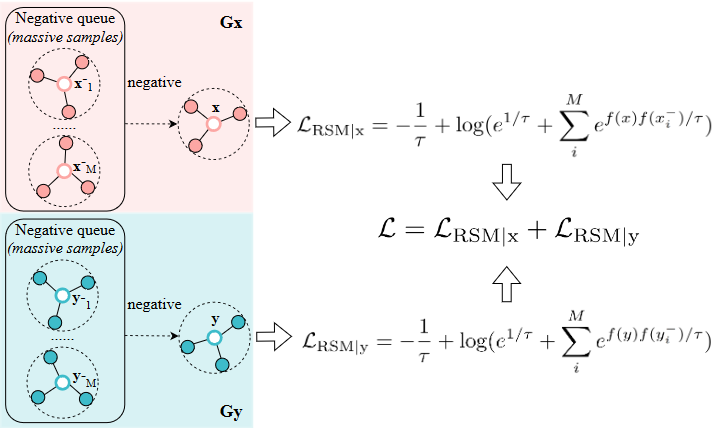
\includegraphics[width = 1\linewidth]{figure/3.png}
    \caption{The training process of SelfKG. It leverages a negative queue for each KG to provide massive negative samples (up to 4k at a time) for calculating the self-supervised contrastive loss.}
    \label{3}
\end{figure}
In practice, the paper jointly optimizes the loss on both $G_x$ and $G_y$ as follows, which is also illustrated in Fig \ref{rsm} (right) and Fig \ref{3}.
\begin{gather}\label{eq5}
    \mathcal{L} = \mathcal{L}_{RSM|\lambda ,X}(f;\tau ,M,p_x) + \mathcal{L}_{RSM|\lambda ,x}(f;\tau ,M,p_y)
\end{gather}
In addition, as the error term of $\mathcal{L}_{\lambda}(f;\tau,M,p_x)$ decays in $O(M^{-\frac{2}{3}})$ (Theorem \ref{2}), the paper uses a comparatively large number of negative samples to boost the performance.
\begin{figure*}[h]
  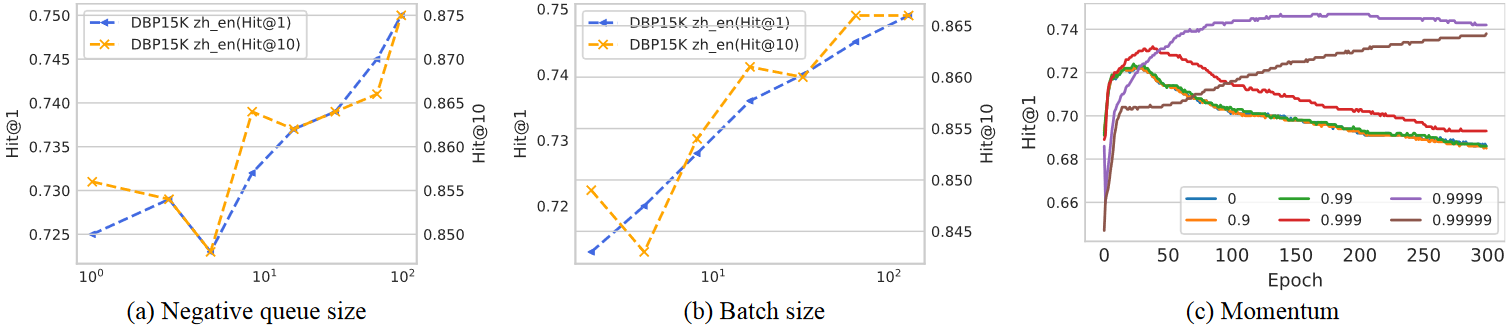
\includegraphics[width=\textwidth]{figure/study.png}
  \caption{Study on (a) negative queue size, (b) batch size, and (c) momentum on DBP15Kzh\_en. (c) presents the test Hit@1 curve throughout the training epochs. \cite{DBLP:journals/corr/abs-2203-01044}}
  \label{study}
\end{figure*}
\subsection{Multiple Negative Queues}
Given that encoding massive negative samples on the fly is quite expensive, increasing the number of negative samples may inevitably result in additional computational costs. We suggest modifying the MoCo technique \cite{he2020momentum} for SelfKG to address this problem. The previously encoded batches are kept in Moco's negative queue, which can accommodate thousands of encoded negative samples for a low cost. We practically keep two negative queues associated with the two input KGs in order to adapt to the self-negative sampling strategy in SelfKG. Fig \ref{3} provides an illustrative example. In the beginning, we would not implement the gradient update until one of the queues reaches the predefined length 1+K where ‘1’ is for the current batch and K is for the number of previous batches used as negative samples. Given $|E|$ as the number of entities in a Knowledge Graph, $K$, and the batch size $N$ are constraint by
\begin{gather}
    (1+K)\times N < min(|E_x|,|E_y|)
\end{gather}
it is guaranteed that we would not sample out entities in the current batch. As a result, the real number of negative samples used for the current batch is $(1+K) \times N-1$.

\noindent \textbf{Momentum update} The main challenge brought by negative queues is the obsolete encoded samples, especially for those encoded at the early stage of training, during which the model parameters vary drastically. Thus, the end-to-end training,  which only uses one frequently-updated encoder, may actually harm the training. To mitigate this, the paper adopts the momentum training strategy, which maintains two encoders-the online encoder and the target encoder. While the online parameter of encoders $\theta_{online}$ is instantly updated with the back-propagation, the target encoder $\theta_{target}$ for encoding the current batch and then pushing into the negative queue is asynchronously updated with momentum by:
\begin{gather}
    \theta _{target}\longleftarrow m \cdot \theta _{target} +(1-m)\cdot\theta _{online},m\in[0,1) 
\end{gather}
A proper momentum is not only important for steady training but may also influence the final performance by avoiding representation collapse.

The paper presents SelfKG for self-supervised entity alignment. Fig \ref{rsm} illustrates that: 1. relative similarity metric (RSM) pushes the non-aligned entities ($y^{-}_0 , y^{-}_1 and y^{-}_2$) of $x$ far enough, instead of directly pulling underlyingly-aligned y close to $x$ (labeled pairs), enabling learning without label supervision; 2. self-negative sampling samples negative entities for $x$ from $G_x$ to avoid sampling the true $y$ as its negative. Fig \ref{3} illustrates the training of SelfKG. It leverages existing techniques—embeddings from pre-trained language models and neighborhood aggregator—to initialize entity embeddings into a uni-space. The technical contributions of SelfKG lie in:
\begin{enumerate}
    \item the design of the self-supervised loss in Eq.\ref{eq2} enabled by our relative similarity metric (RSM) in Knowledge Graphs.
    \item the strategy of self-negative sampling that furthers Eq. \ref{eq2} into Eq.\ref{eq5} to avoid false-negative samples.
    \item the extension of MoCo to two negative queues to support an efficient usage of massive negative samples.
\end{enumerate}
\section{Thesis Reproduction}
In this section, I will describe the code of the paper in more detail and show the results.
\subsection{Overall framework}
As shown in the Fig \ref{code overview}, the code reproduced in the paper is as follows. The data folder stores DBP15K and DWY100K which are two datasets that can be obtained through the getdata.sh file. DBP15K is a multilingual database that contains entity-relation-entity triples in 15 different languages. It is used for research in the field of natural language processing, specifically for tasks related to cross-lingual knowledge base alignment and entity linking. DWY100k is a dataset of 100,000 Wikipedia articles in English that have been annotated for the presence of named entities and the relationships between them. It is used for research in the field of natural language processing, specifically for tasks related to named entity recognition and relation extraction.

In the main file, run\_DWY\_LaBSE\_neighbor.py and

\noindent run\_LaBSE\_neighbor.py are calling the training files for different datasets in the model folder, respectively, and running the trainer class. In addition to those two training files for different training sets in the model folder, there are two layers\_ LaBSE\_SSL.py and layers\_LaBSE\_SSL\_DWY.py are what the original paper used to do the ablation studys.

In the preprocess folder, there are some preprocessing operations on the original dataset, such as "deal\_dataset", "get\_token", "neighbor\_token", etc.
\begin{figure}[H]
    \centering
    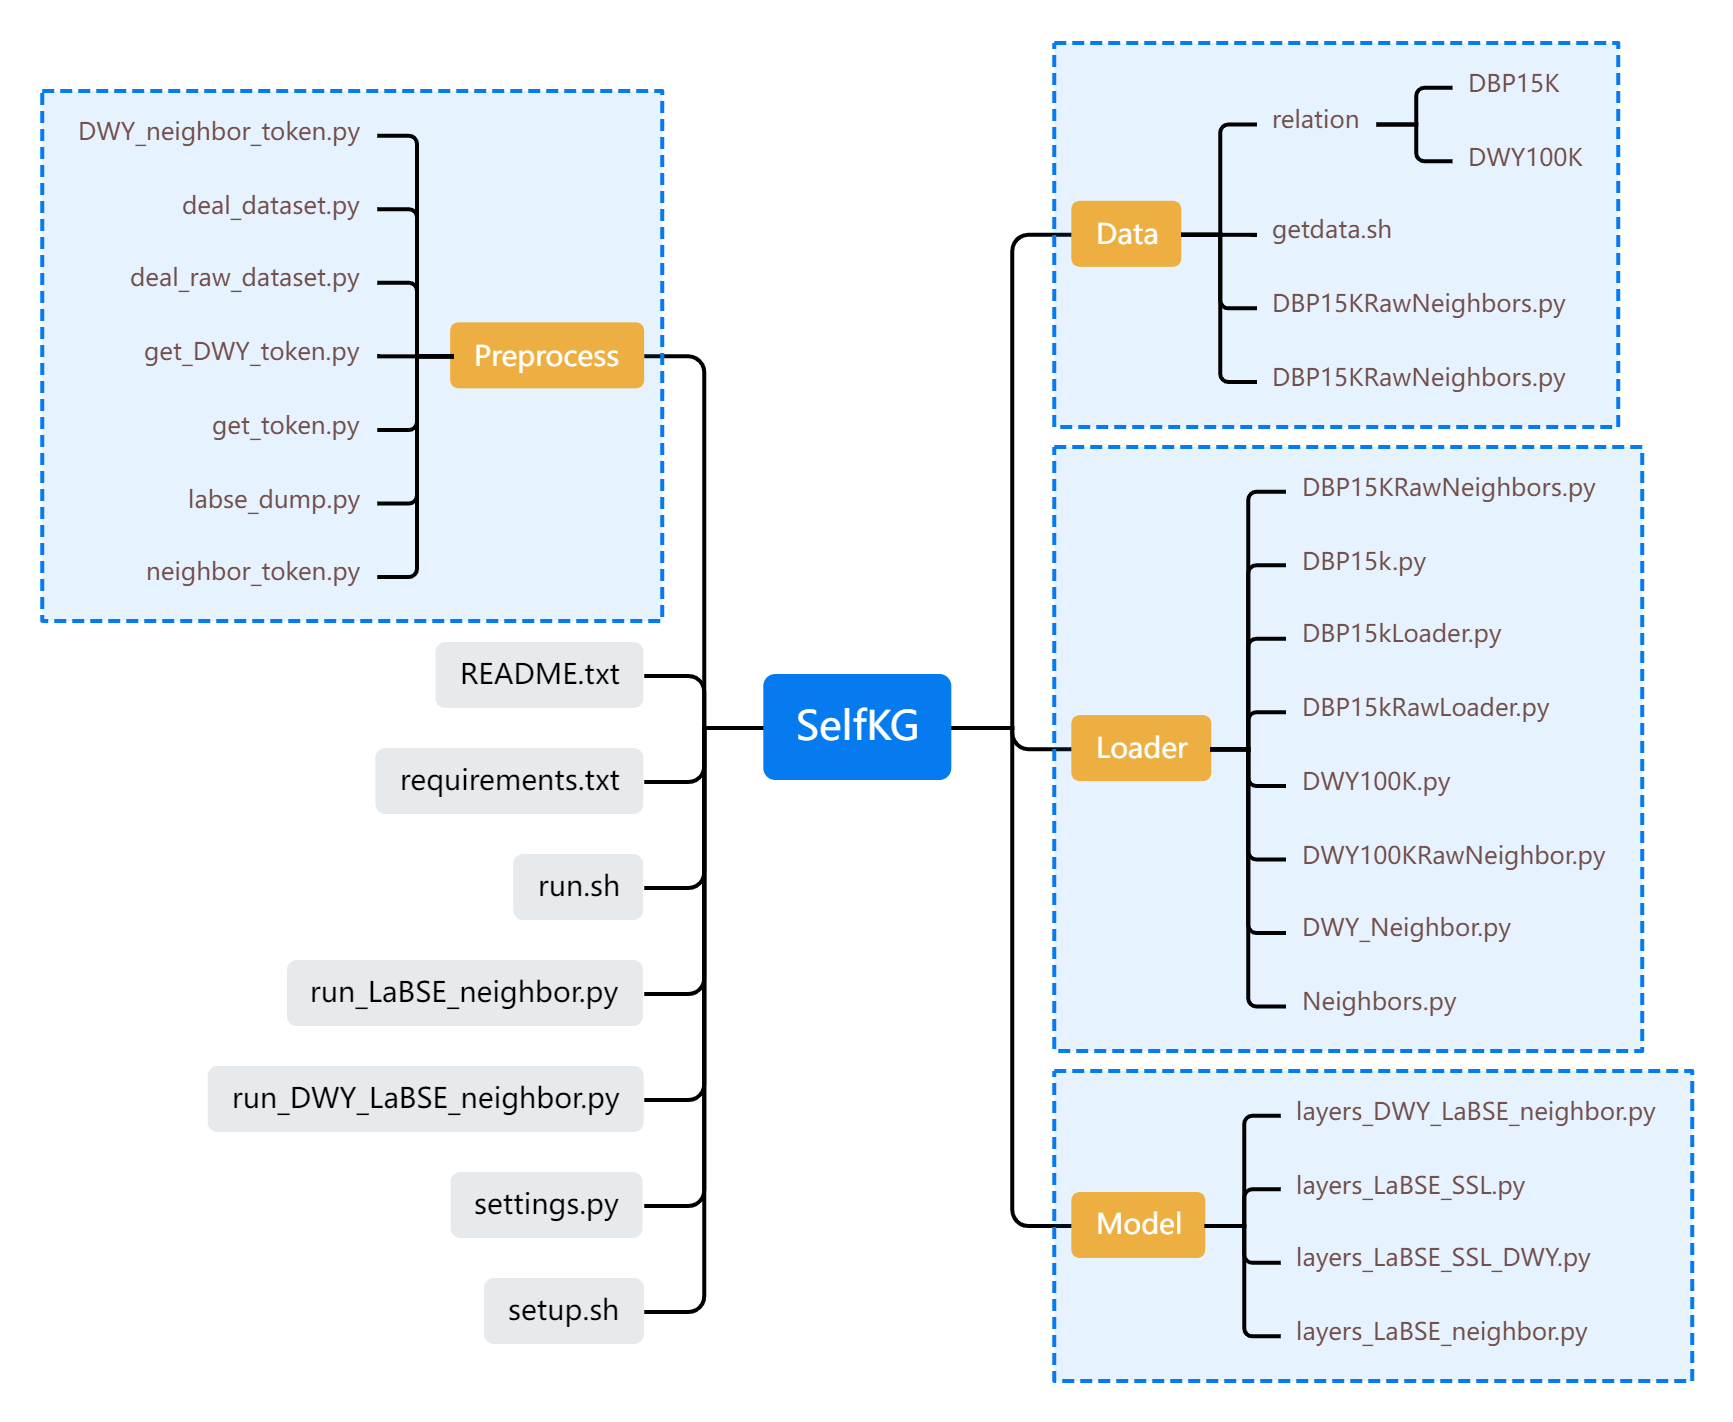
\includegraphics[height=0.88\linewidth]{figure/SelfKG.png}
    \caption{Overview framework of code}
    \label{code overview}
\end{figure}
\subsection{Detail Analysis}
\begin{figure*}[h]
    \centering
    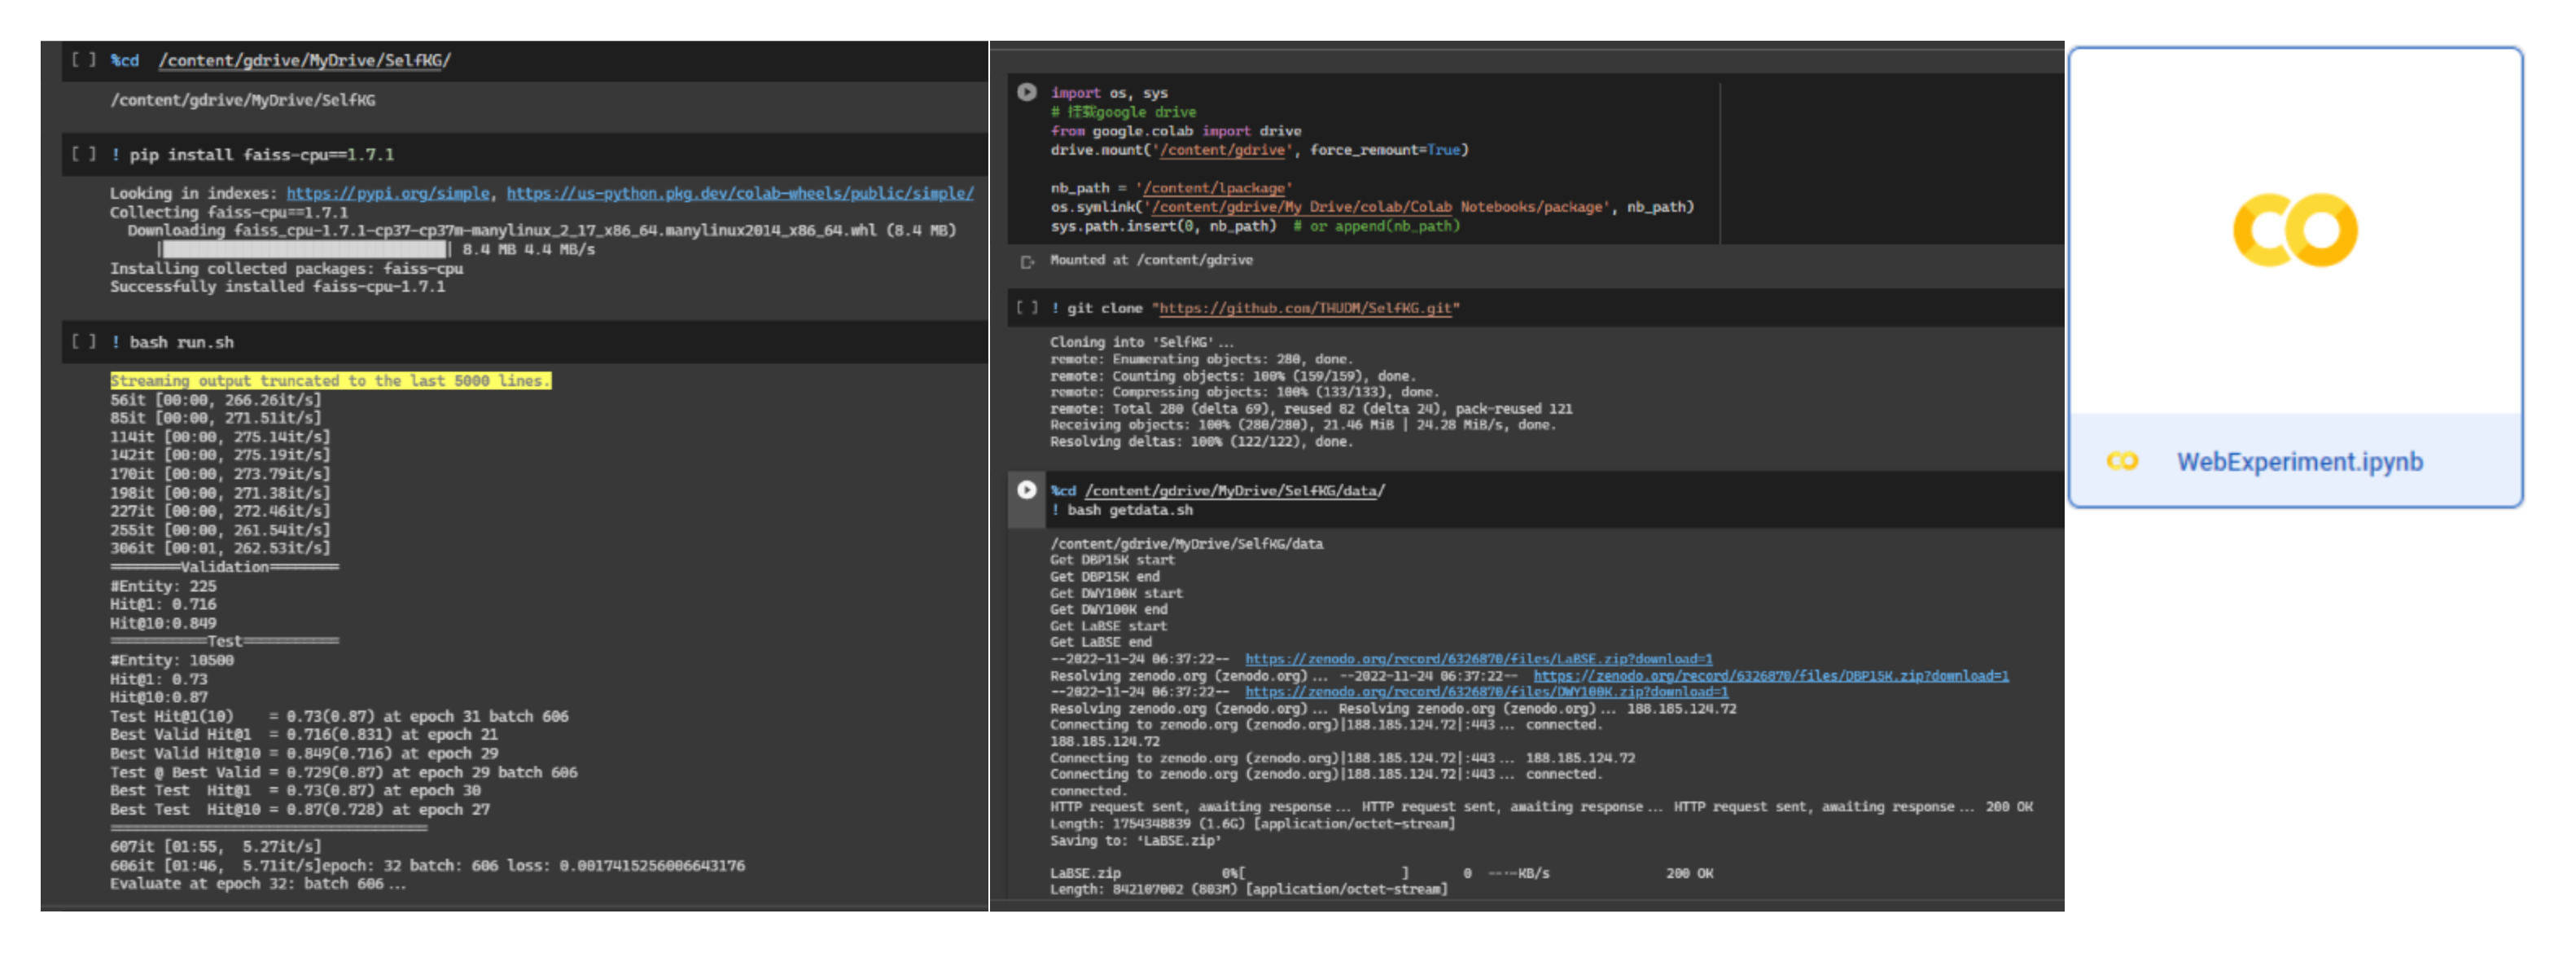
\includegraphics[width=1\linewidth]{figure/code.png}
    \caption{Preprocess of experiment}
    \label{code}
\end{figure*}
I adapted Google's Colab as our experimental environment, as shown in Fig \ref{code}. The Python third-party libraries needed to complete the experiment are listed below:
\begin{enumerate}
    \item  torch==1.9.0 or above
    \item  faiss-cpu==1.7.1 or above
    \item  numpy==1.19.2 or above
    \item  pandas==1.0.5 or above
    \item  tqdm==4.61.1 or above
    \item  torchtext==0.10.0 or above
    \item  transformers==4.8.2 or above
\end{enumerate}
And in the two training files, certain parameters can be setting. As shown in Fig \ref{parse}.
\begin{figure}
    \centering
    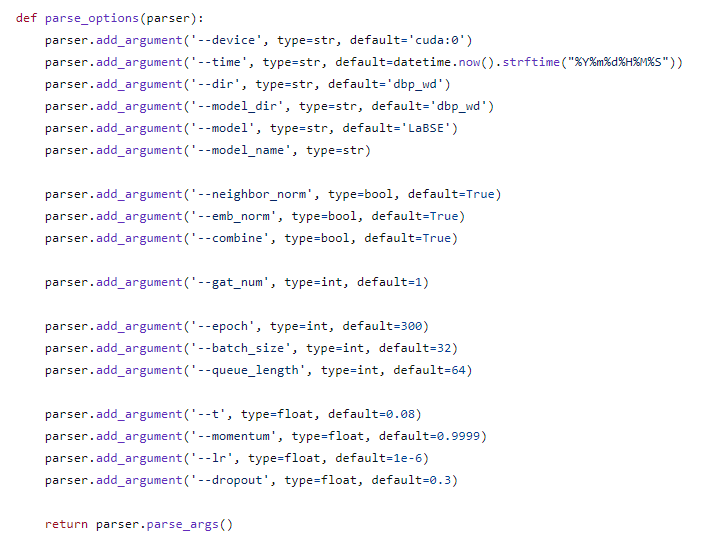
\includegraphics[width=1\linewidth]{figure/parse.png}
    \caption{Setting}
    \label{parse}
\end{figure}
\begin{figure}
    \centering
    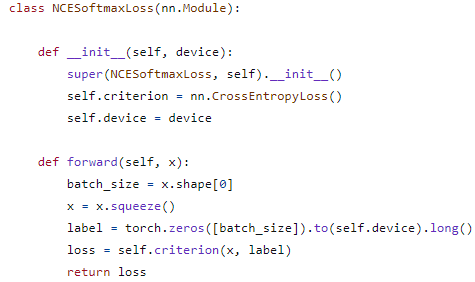
\includegraphics[width=1\linewidth]{figure/loss.png}
    \caption{Contrastive loss}
    \label{loss}
\end{figure}
Here we can see that the experiment has a batch size of 64, default training epochs of 300, a learning rate of 0.0001, and a dropout of 0.3. Also in the two training files, they include graph-attention mechanism, as showin in Fig \ref{gat}.
\begin{figure}
    \centering
    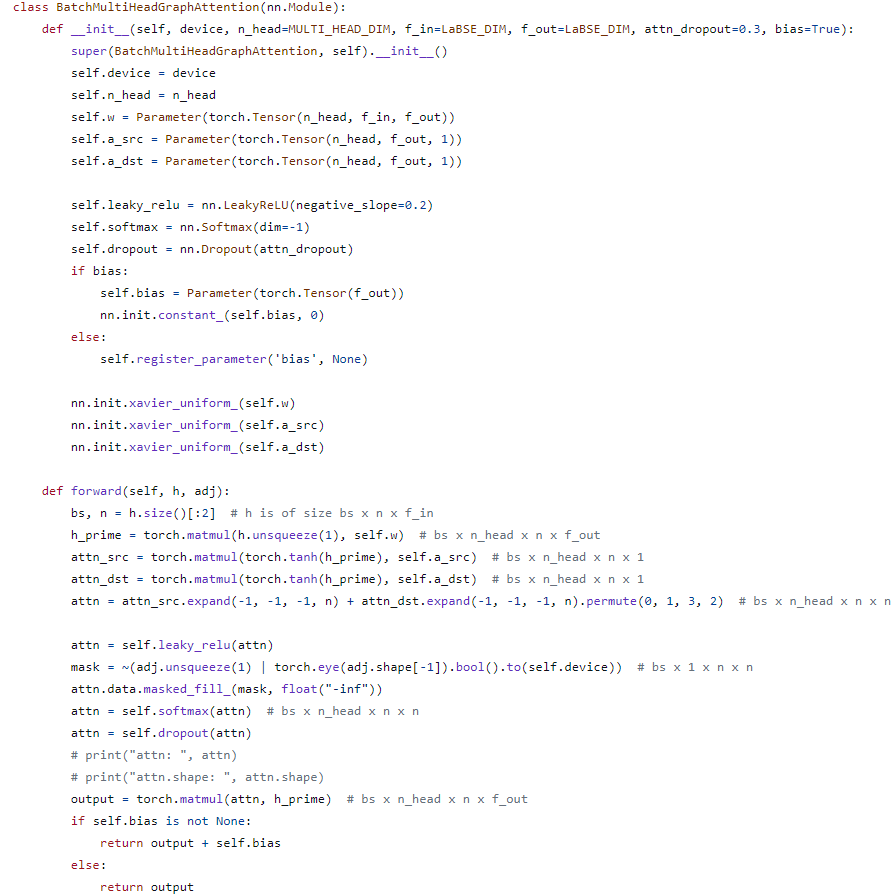
\includegraphics[width=1\linewidth]{figure/graphattention.png}
    \caption{Code of Graph-attention mechanism}
    \label{gat}
\end{figure}
\subsection{Training results}
The unique nohup command was used to save the output results to an .out file. The initial training is shown in the Fig \ref{begin}, and the results after 150 epochs of training are shown in the Fig \ref{stop}.
\begin{figure}
    \centering
    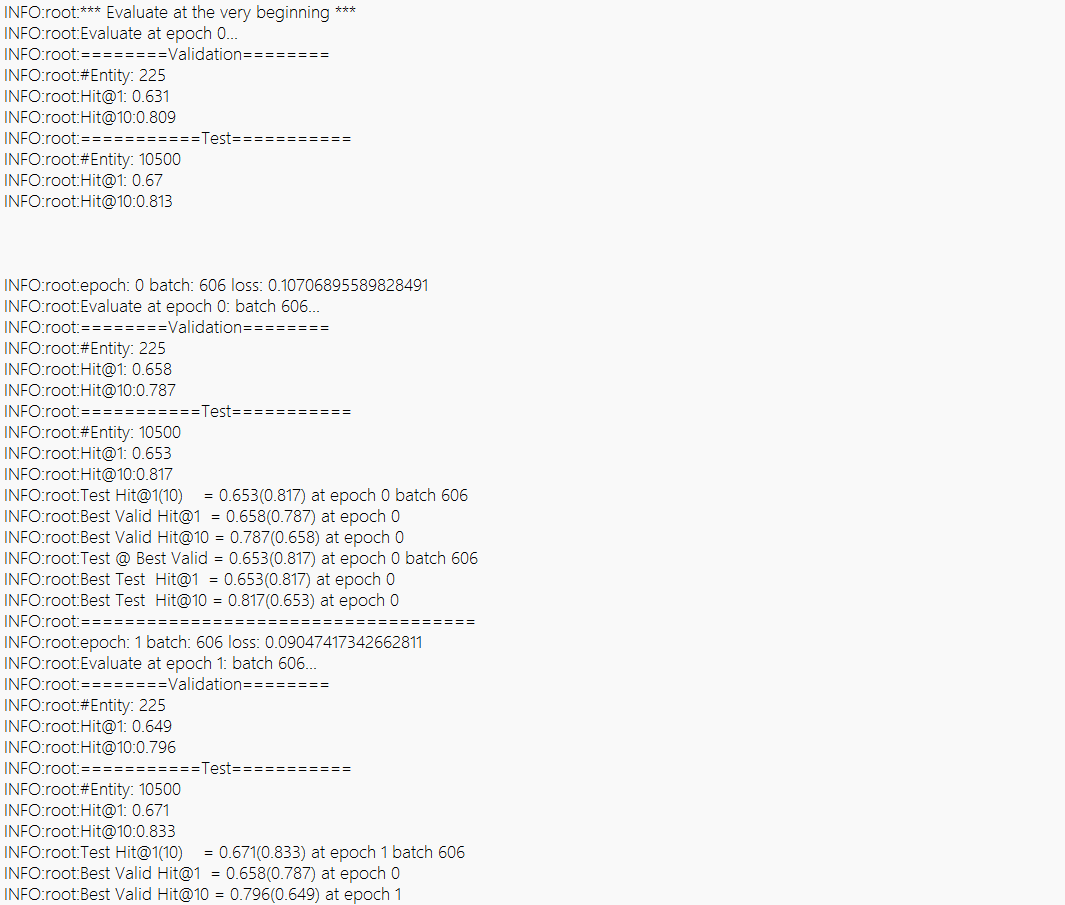
\includegraphics[width=1\linewidth]{figure/b.png}
    \caption{Training beginning}
    \label{begin}
\end{figure}
\begin{figure}
    \centering
    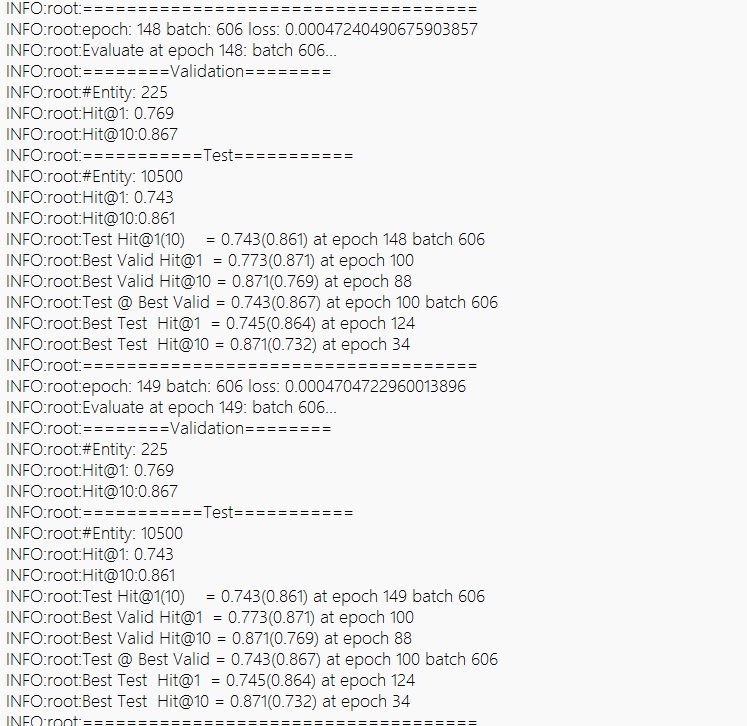
\includegraphics[width=1\linewidth]{figure/e.png}
    \caption{Training stop}
    \label{stop}
\end{figure}

The experiment is trained separately for the cases under two datasets, each with 150 epochs, and the epochs with the best final HITS@1 and HITS@10 scores are selected. For both experiments on DWY100K and DBP15K, the paper randomly selects 5\% links from the training set in the original datasets as our validation set and evaluate their model’s performance both on the validation set and the testing set. They stop the training progress once our model reaches the best performance on the validation set and record Hit@1 and Hit@10 results on the testing set, which approximately around 150 epochs. In Fig \ref{metric}, shows the coding part of metric.
\begin{figure}
    \centering
    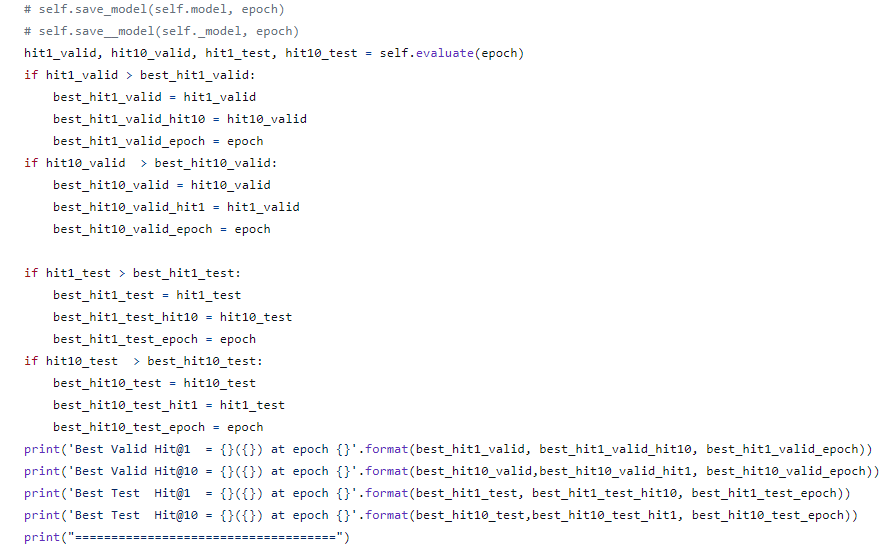
\includegraphics[width=1\linewidth]{figure/metric.png}
    \caption{Code of metric}
    \label{metric}
\end{figure}

\section{EXPERIMENT}

We evaluate SelfKG on two widely-acknowledged public benchmarks: DWY100K and DBP15K. DWY100K is a monolingual dataset and DBP15K is a multi-lingual dataset.

{\bfseries DWY100K}. The DWY100K dataset used here is originally built by [31]. DWY100K consists of two large datasets: 

\begin{itemize}
\item $DWY100K_{dbp\_wd}$ (DBpedia to Wikidata) 
\item $DWY100K_{Kdb\_yg}$ (DBpedia to YAGO3)
\end{itemize}

Each dataset contains 100,000 pairs of aligned entities. However, the entity in the "wd" (Wikidata) part of $DWY100K_{dbp\_wd}$ are represented by indices (e.g., Q123) instead of URLs containing entity names, and we search their entity names via the Wikidata1 API for python.

{\bfseries DBP15K}. The DBP15K dataset is originally built by [30]2 and translated into English by [42]. The DBP15K consists of three crosslingual datasets:
\begin{itemize}
\item $DBP15K_{zh\_en}$ (Chinese to English)
\item $DBP15K_{ja\_en}$ (Japanese to English) 
\item $DBP15K_{fr\_en}$ (French to English)
\end{itemize}

All three datasets are created from multi-lingual DBpedia, and each contains 15,000 pairs of aligned entities. We report results on both original and translated version.

The statistics of DWY100K and DBP15K we use in our work are shown in Table 1. Beyond basic information, we also present a study on datasets’ average (1-hop) neighbor similarity, which is the ratio of aligned neighbors of a pair of aligned entities, indicating how noisy the neighborhood information is. We observe that DWY100K’s neighborhood information is quite useful, while DBP15K’s neighborhood information can be very noisy.

Experiment Setup. We follow the original split of DWY100K [31] and DBP15K [30] which are shown in Table 1. For SelfKG, we randomly take out 5$\%$ from the original training set as a dev set for early stopping. We use Hit\@k (k = 1, 10) to evaluate our model’s performance as most works do. The similarity score is calculated using the $\mathscr{l}_{2}$ distance of two entity embeddings. The batch size is set to 64, momentum m is set to 0.9999, temperature $\tau$ is set to 0.08, and queue size is set to 64. We use a learning rate of 10-6 with Adam on a Ubuntu server with NVIDIA V100 GPUs (32G).

\begin{table}
\caption{Statistics of DWY100K and DBP15K.}
\label{tab:freq}
\linespread{2}
\renewcommand\arraystretch{1.5}
\scalebox{0.9}{
\begin{tabular}{ccccccc} %需要10列
\toprule %添加表格头部粗线
\multicolumn{1}{c}{\multirow{2}{*}{Model}}& \multicolumn{2}{c}{DWY100K} &\multicolumn{3}{c}{DBP15K}\\
\multicolumn{1}{c}{}&dbp\_wd&dbp\_yg&zh\_en&ja\_en&fr\_en\\  %有n个&,就表示该行有n+1列
\midrule %绘制一条水平横线
\multicolumn{1}{c}{\#Link}& 99990& 100000 &15000& 15000& 15000\\   % 占两列,列名为A;后面陆续跟着数字
\multicolumn{1}{c}{\#Test Link}&69993 &70000 & 10500 & 10500 & 10500 \\
\multicolumn{1}{c}{neighbor similarity}&0.633 &0.777 &0.418&0.188 &0.182\\
\bottomrule %添加表格底部粗线
\end{tabular}
}
\end{table}

%%=================================================================================
\subsection{Baseline introduction of DWY100K dataset}

In this section, we report the results of the DWY100K baseline. For all baselines, we obtain report scores from the corresponding papers. According to the use proportion of training labels, we divide all models into two types:

\begin{itemize}
\item Supervised: 100$\%$ of the aligned entity links in the training set is leveraged.
\item Unsupervised $\&$ Self-supervised: 0$\%$ of the training set is leveraged.
\end{itemize}

\subsubsection{MTransE \cite{chen2016multilingual}}

Many recent works have demonstrated the benefits of knowledge graph embeddings in completing monolingual knowledge graphs. Inasmuch as related knowledge bases are built in several different languages, achieving cross-lingual knowledge alignment will help people in constructing a coherent knowledge base, and assist machines in dealing with different expressions of entity relationships across diverse human languages. Unfortunately, achieving this highly desirable crosslingual alignment by human labor is very costly and error-prone. 

MTransE model is a multi language knowledge map embedding model based on translation. By encoding entities and relations of each language in a separated embedding space, MTransE provides transitions for each embedding vector to its cross-lingual counterparts in other spaces, while preserving the functionalities of monolingual embeddings.

This model uses the combination of two component models (namely, knowledge model and alignment model) to learn the graphical structure of multilingual knowledge.The knowledge model encodes entities and relations in a language-specific version of knowledge graph.

We explore the method that organizes each language-specific version in a separated embedding space, in which MTransE adopts TransE as the knowledge model. On top of that, the alignment model learns cross-lingual transitions for both entities and relations across different embedding spaces, where the following three representations of cross-lingual alignment are considered: distance-based axis calibration, translation vectors, and linear transformations.

\subsubsection{JAPE \cite{sun2017cross}}

Entity alignment is the task of finding entities in two knowledge bases (KBs) that represent the same real-world object. When facing KBs in different natural languages, conventional cross-lingual entity alignment methods rely on machine translation to eliminate the language barriers. These approaches often suffer from the uneven quality of translations between languages. While recent embedding-based techniques encode entities and relationships in KBs and do not need machine translation for cross-lingual entity alignment, a significant number of attributes remain largely unexplored. JAPE model is a joint attribute storage embedded model for cross language entity alignment.

It jointly embeds the structures of two KBs into a unified vector space and further refines it by leveraging attribute correlations in the KBs. It employs two modules, namely structure embedding (SE) and attribute embedding (AE), to learn embeddings based on two facets of knowledge (relationship triples and attribute triples) in two KBs, respectively. SE focuses on modeling relationship structures of two KBs and leverages existing alignment given beforehand as bridge to overlap their structures. AE captures the correlations of attributes (i.e. whether these attributes are commonly used together to describe an entity) and clusters entities based on attribute correlations. Finally, it combines SE and AE to jointly embed all the entities in the two KBs into a unified vector space Rd, where d denotes the dimension of the vectors. The purpose of the JAPE model is to find the potential cross language target entity of the source entity (that is, the truly aligned entity we want to find) by searching the nearest neighbor in Rd. We expect the embedding of potentially aligned cross language entities to be close to each other.

In conclusion, the JAPE model has the following characteristics:
\begin{itemize}
\item JAPE model is an embedded based cross language entity alignment method, which does not rely on machine translation between cross language knowledge bases.
\item The JAPE model jointly embeds the relational triplet of the two knowledge bases through structural embedding, and further refines the embedding by using the attribute triplet and attribute embedding of the knowledge base.
\end{itemize}

\subsubsection{IPTransE \cite{zhu2017iterative}}

Entity alignment aims to link entities and their counterparts among multiple knowledge graphs (KGs). Most existing methods typically rely on external information of entities such as Wikipedia links and require costly manual feature construction to complete alignment. The IPTransE model is a new method of entity alignment through joint knowledge embedding. It jointly encodes both entities and relations of various KGs into a unified low-dimensional semantic space according to a small seed set of aligned entities. During this process, we can align entities according to their semantic distance in this joint semantic space. 

More specifically, The IPTransE model consists of three parts: 
\begin{itemize}
\item{\bfseries Knowledge Embeddings.} We learn both entity and relation embeddings following the translation-based KRL methods according to the triple facts in various KGs.
\item{\bfseries Joint Embeddings.} We learn to map knowledge embeddings of various KGs into a joint semantic space according to a seed set of known aligned entities. 
\item{\bfseries Iterative Alignment.} We iteratively align entities and their counterparts and update the joint knowledge embeddings by taking those high-confident aligned entities increasingly found by our method into consideration.
\end{itemize}

\subsubsection{GCN-Align \cite{wang2018cross}}

Multilingual knowledge graphs (KGs) such as DBpedia and Y AGO contain structured knowledge of entities in several distinct languages, and they are useful resources for cross-lingual AI and NLP applications. Cross-lingual KG alignment is the task of matching entities with their counterparts in different languages, which is an important way to enrich the crosslingual links in multilingual KGs. GCN-Align model is a new method of cross language KG alignment through graph convolution network (GCN). Entity alignments are discovered based on the distances between entities in the embedding space. Embeddings can be learned from both the structural and attribute information of entities, and the results of structure embedding and attribute embedding are combined to get accurate alignments.

GCN-Align model directly models the equivalence relationship between entities by using graph convolution network (GCN). GCN is a kind of convolutional network which directly operates on graphstructured data; it generates node-level embeddings by encoding information about the nodes’ neighborhoods. The adjacency of two equivalent entities in KGs usually includes other equivalent entities, so GCN-Align model selects GCN to generate neighborhood aware embeddings of entities, which are used to discover entity alignment. GCN-Align model can also provide a simple and effective method to include entity attribute values in the aligned model. More specifically, the GCN-Align model has the following advantages:
\begin{itemize}
\item GCN-Align model uses the entity relations in each KG to build the network structure of GCNs, and it only considers the equivalent relations between entities in model training. GCN-Align model has small model complexity and can achieve encouraging alignment results.
\item GCN-Align model only needs pre-aligned entities as training data, and it does not require any pre-aligned relations or attributes between KGs.
\item Entity relations and entity attributes are effectively combined in GCN-Align model to improve the alignment results.
\end{itemize}

\subsubsection{MuGNN \cite{cao2019multi}}

Entity alignment typically suffers from the issues of structural heterogeneity and limited seed alignments. MuGNN model is a new multi-channel graphical neural network model, which learns alignment oriented knowledge graph (KG) embedding by robust coding two KG through multi-channel. Each channel encodes KGs via different relation weighting schemes with respect to self-attention towards KG completion and cross-KG attention for pruning exclusive entities respectively, which are further combined via pooling techniques. Moreover, MuGNN model is expected to reconcile the structural differences of two KGs, and thus make better use of seed alignments.

The MuGNN model jointly implements KG reasoning and alignment to clearly coordinate the structural differences between different KGs, and uses the graph based model to better utilize the seed alignment information. The MuGNN model can encode different KGs to learn alignmentoriented embeddings. For each KG, MuGNN utilizes different channels towards KG completion and pruning, so as to reconcile two types of structural differences: missing relations and exclusive entities. Different channels are combined via pooling techniques, thus entity embeddings are enhanced with reconciled structures from different perspectives, making utilization of seed alignments effectively and efficiently. Between KGs, each channel transfers structure knowledge via shared parameters.

The main characteristics of MuGNN model are as follows:
\begin{itemize}
\item MuGNN model is a new multi-channel GNN model, which learns alignment oriented embedding by coding graphs from different angles (completion and pruning), so it is robust to structural differences.
\item The MuGNN model jointly implements KG reasoning and alignment, so that it can be completed through rule reasoning and transfer, and pruning through cross KG attention to clearly coordinate the heterogeneity of KG.
\end{itemize}

\subsubsection{RSNs \cite{guo2019learning}}

Recursive skip network (RSN) uses skip mechanism to bridge the gap between entities. RSNs integrate recurrent neural networks (RNNs) with residual learning to efficiently capture the long-term relational dependencies within and between KGs. We design an end-to-end framework to support RSNs on different tasks.

Instead of learning the embeddings in a triple-level view, RSNs concentrate on learning from relational paths. A relational path is defined as an entity-relation chain, such as (United Kingdom, country-, Tim BernersLee, employer, W3C), where country- is a reverse relation that we create additionally to enhance the connectivity. It is clear that paths can provide richer relational dependencies than triples without losing the local relational information of entities. RSNs also overcome the limitations that many existing methods are only designed for one specific task of KG embedding. 

In KGs, subject entities are vital for inferring a specific object entity. The local neighbor information would be broken if we use RNNs to model relational paths. To overcome this weakness, RSNs enable the output hidden states of relations to learn a residual from their direct subject entities when inferring object entities, with only a few more parameters.

\subsubsection{BootEA \cite{sun2018bootstrapping}}

Embedding-based entity alignment represents different knowledge graphs (KGs) as low-dimensional embeddings and finds entity alignment by measuring the similarities between entity embeddings. Existing approaches have achieved promising results, however, they are still challenged by the lack of enough prior alignment as labeled training data. BootEA model is a bootstrap method based on embedded entity alignment. It iteratively labels likely entity alignment as training data for learning alignment-oriented KG embeddings. Furthermore, it employs an alignment editing method to reduce error accumulation during iterations.

BootEA model is a bootstrapping approach for entity alignment. Bootstrapping is a widely-used semi-supervised learning technique. It iteratively trains a classifier by bootstrapping from both labeled and unlabeled data. 

The main features of the BootEA model are as follows:
\begin{itemize}
\item The BootEA model models entity alignment as a classification problem, which seeks to maximize the alignment possibility of all marked and unmarked entities embedded based on KG.
\item For alignment oriented KG embedding, BootEA model proposes an objective function based on limit, which expects positive triples to score lower while negative triples score higher. The BootEA model also exchanges aligned entities between triples of different KGs to align the embedding in a unified space.
\item To overcome the lack of sufficient training data, the BootEA model updates the alignment oriented embedding by marking possible alignments and iteratively adding them to the training data. It marks possible alignment based on the global optimal goal to ensure accuracy, and uses alignment editing methods to reduce error accumulation.
\end{itemize}

\subsubsection{NAEA \cite{zhu2019neighborhood}}

Multilingual knowledge graphs constructed by entity alignment are the indispensable resources for numerous AI-related applications. Most existing entity alignment methods only use the triplet-based knowledge to find the aligned entities across multilingual knowledge graphs, they usually ignore the neighborhood subgraph knowledge of entities that implies more richer alignment information for aligning entities.

NAEA model is a kind of neighborhood aware attention representation method for multilingual knowledge graph, which combines the level information of neighborhood subgraphs of entities. NAEA devises an attention mechanism to learn neighbor-level representation by aggregating neighbors’ representations with a weighted combination. The attention mechanism enables entities not only capture different impacts of their neighbors on themselves, but also attend over their neighbors’ feature representations with different importance.

NAEA are composed of knowledge embedding component KE and entity alignment component EA. Both KE and EA components incorporate neighbor-level and relation-level information with different weights for learning KGs’ embedding representation and aligning entities respectively. KE component devises an attention mechanism to obtain neighbor-level representation by aggregating neighbors with a weighted combination, and uses the triplet-based characteristic information to learn relation-level representation. EA component determines alignments between entities across multilingual KGs by measuring the similarity of their integrated representations, which are also fused from neighbor-level and relation-level representations with different weights.

The main features of the NAEA model are as follows:
\begin{itemize}
\item NAEA combines neighborhood level and relationship level feature information in the knowledge graph to perform multilingual entity alignment tasks.
\item The KE component designed a neighbor aware attention mechanism by aggregating neighbor embeddings with different impacts to learn neighbor level representation.
\item EA components perform entity alignment through the similarity of entity integration representations, which integrates neighborhood level and relationship level feature representations.
\end{itemize}

\subsubsection{TransEdge \cite{sun2019transedge}}

Learning knowledge graph (KG) embeddings has received increasing attention in recent years. Most embedding models in literature interpret relations as linear or bilinear mapping functions to operate on entity embeddings. However, such relation-level modeling cannot capture the diverse relational structures of KGs well. TransEdge model is a new edge centered embedded model, which represents the upper and lower cultural relations according to specific head and tail entity pairs. 

This model distinguishes the representation of relationships between specific contexts of different entities. One head-tail entity pair can hold different relations, i.e, one edge can have different labels. Also, different edges can have the same label, indicating that there are multiple head-tail entity pairs having the same relation. Thus, it is intuitive that entities should have explicit embeddings while relations should have different contextualized representations when translating between different head-tail entity pairs. Therefore, the TransEdge model embeds the upper and lower cultures into different edges. The context of a relationship is specified by its head and tail entities. In order to capture the KG structure, TransEdge model follows the idea of translational KG embedding, and uses edge embedding to build the transformation between entity embedding.
The main features of the TransEdge model are as follows:
\begin{itemize}
\item Different from the existing models, TransEdge learns to embed KG by representing the upper and lower cultural relationships according to specific head and tail entity pairs.
\item TransEdge provides a new perspective for KG embedding.
\end{itemize}

\subsubsection{RDGCN \cite{wu2019relation}}

Entity alignment is the task of linking entities with the same real-world identity from different knowledge graphs (KGs), which has been recently dominated by embedding-based methods. Such approaches work by learning KG representations so that entity alignment can be performed by measuring the similarities between entity embeddings.

RDGCN model is a new relationship aware dual graph convolution network, which combines relationship information through the concern interaction between knowledge graph and its dual relationship counterpart, and further captures adjacent structures to learn better entity representation.

As a departure from GCNs and R-GCNs, RDGCN model allows multiple rounds of interactions between the primal entity graph and its dual relation graph, enabling the model to effectively incorporate more complex relation information into entity representations. 

\subsubsection{COTSAE \cite{yang2020cotsae}}

Entity alignment is a fundamental and vital task in Knowledge Graph (KG) construction and fusion. Previous works mainly focus on capturing the structural semantics of entities by learning the entity embeddings on the relational triples and pre-aligned ”seed entities”. Some works also seek to incorporate the attribute information to assist refining the entity embeddings. However, there are still many problems not considered, which dramatically limits the utilization of attribute information in the entity alignment. Different KGs may have lots of different attribute types, and even the same attribute may have diverse data structures and value granularities. Most importantly, attributes may have various ”contributions” to the entity alignment. To solve these problems, the COTSAE model combines the structure and attribute information of entities by jointly training two embedded learning components. 

There are still many problems in the use of entity attribute information for embedding-based entity alignment: 
\begin{itemize}
\item The attribute information is pretty challenging to use as different KGs may have lots of different attribute types, and the name of the same attribute type may also be different due to naming conventions. Attribute values are diverse in data structure and value granularity.
\item Different attributes contributes differently to the entity alignment, and there are often a large number of ”noise” attributes that are unrelated to the entity alignment but interfering with the alignment.
\item Attribute and structure information describes the internal and external semantics of an entity, and they are independent of each other in the KGs. Actually, there are different emphasis on these two information in different KGs.
\end{itemize}

The structure information of some KGs may be sparse, or some KGs may be lack of attribute information. If learning them into one unified embedding space by constraining the embeddings from different information consistent,  sparse structure information will limit the learning of structure embedding, which definitely affects the learning of attribute embedding.

The COTSAE model is used to solve the above challenges. It is a joint training model consisting of two embedded components for integrating structure and attribute information. One component is the KG representation learning model TransE to learn the structural embedding of entities. The other component is a novel Pseudo-Siamese network with joint attention to learn the weights of attributes and bi-directional gated recurrent unit encoder (Bi-GRU) to characterize attribute values. In COTSAE, both structure and attribute information can be used to generate possible entity alignment, for example, when the structure information of KGs is difficult to get new entity alignments, the attribute information can be used to complement it for further entity alignment. Similarly, when the attribute information is insufficient, the structure information can also assist it in the entity alignment. 

\subsubsection{BERT-INT \cite{tang2020bert}}

Knowledge graph alignment aims to link equivalent entities across different knowledge graphs. To utilize both the graph structures and the side information such as name, description and attributes, most of the works propagate the side information especially names through linked entities by graph neural networks. However, due to the heterogeneity of different knowledge graphs, the alignment accuracy will be suffered from aggregating different neighbors. BERT-INT model is an interactive model that only uses auxiliary information. It does not gather neighbors, but calculates interactions between neighbors, which can capture fine-grained matching of neighbors. Similarly, the interaction of attributes is modeled.

We propose the BERT-INT model to use only edge information in a unified way, especially the names/descriptions of current entities and neighbors and the attributes of current entities. Generally, we mimic the cognitive process of comparing two entities by humans, who usually first compare current entities and then continue to check whether there are similar neighbors. Following this, based on the embedding of any piece of name, description and attribute, we compare each pair of neighbors or attributes, referred to as interactions henceforth, instead of aggregating them. In this way, we can capture the fine-grained exact/semantic matches between neighbors and get rid of the negative influence from the dissimilar neighbors.

Although BERT-INT model leverage the side information of neighbors, unlike the variant GCN models, the structural characteristics of KGs are totally ignored in BERT-INT model, because BERT-INT model never propagate the information of neighbors in graphs. Just because of this, BERT-INT is capable of inductive learning, i.e., we can train BERT-INT on two aligned KGs and apply it to predict the matches between unseen entities in other KGs. However, if adopting the variant GCN models, the test entities should be included in the training KGs.

\subsubsection{CEAFF \cite{zeng2020collective}}

Entity alignment (EA) identifies entities that refer to the same real-world object but locate in different knowledge graphs (KGs), and has been harnessed for KG construction and integration. When generating EA results, current solutions treat entities independently and fail to take into account the interdependence between entities. The CEAFF model first uses three representative features, namely, structure, semantics and string signals, which are suitable for capturing the similarities in different aspects between entities in heterogeneous KGs. In order to make a collective EA decision, CEAFF model describes EA as a classical stable matching problem, which is further effectively solved by delayed acceptance algorithm.

The CEAFF model first uses structural, semantic, and string level features to capture the similarities in different aspects between entities in the source and target KG. These features are representative and widely available. They are effectively modeled and adjusted through the feature generation strategy proposed by CEAFF model. Then, in order to capture the interdependence between EA decisions, CEAFF model describes EA as a classic stable matching problem, and constructs entity preference list by using these features. This problem is further solved by an efficient delayed acceptance algorithm.

\subsubsection{MultiKE \cite{zhang2019multi}}

Previous works mainly focus on the relational structure of entities. Some further incorporate another type of features, such as attributes, for refinement. However, a vast of entity features are still unexplored or not equally treated together, which impairs the accuracy and robustness of embedding-based entity alignment. The MultiKE model unifies multiple views of entities to learn about embedding for entity alignment. Specifically, the MultiKE model uses multiple combination strategies to embed entities based on entity name, relationship and attribute views.

The basic idea of the MultiKE model is to divide various features of KGs into multiple subsets (called views) that complement each other.

%%=================================================================================
\subsection{Baseline introduction of DBP15K dataset}

\subsubsection{SEA \cite{pei2019semi}}

Entity alignment associates entities in different knowledge graphs if they are semantically same, and has been successfully used in the knowledge graph construction and connection. Most of the recent solutions for entity alignment are based on knowledge graph embedding, which maps knowledge entities in a low-dimension space where entities are connected with the guidance of prior aligned entity pairs. The SEA model focuses on two important issues that limit the accuracy of current entity alignment solutions:
\begin{itemize}
\item labeled data of priorly aligned entity pairs are difficult and expensive to acquire, whereas abundant of unlabeled data are not used;
\item knowledge graph embedding is affected by entity’s degree difference, which brings challenges to align high frequent and low frequent entities. 
\end{itemize}

SEA model is a semi supervised entity alignment method (SEA), which is used to align labeled entities with a large amount of unmarked entity information.

SEA model takes advantages of both aligned with unaligned entities, which are represented in low-dimension space by knowledge graph embedding with awareness of the degree difference. In particular, the impact of degree difference is mitigated by an adversarial training, which prevents entities with similar degree from being aggregated into the same region in the embedding space during training. SEA model also design a cycle-consistency based translation loss using the unaligned entities to reduce the search space when learning the mappings. Thus, the learned mappings can better align the entity in one knowledge graph to the corresponding entity in another knowledge graph.

\subsubsection{KECG \cite{li2019semi}}

Entity alignment aims at integrating complementary knowledge graphs (KGs) from different sources or languages, which may benefit many knowledge-driven applications. It is challenging due to the heterogeneity of KGs and limited seed alignments. KECG model is a semi supervised entity alignment method based on knowledge embedding model and cross graph model. It can make better use of seed alignments to propagate over the entire graphs with KG-based constraints. Specifically, as for the knowledge embedding model, KECG model utilize TransE to implicitly complete two KGs towards consistency and learn relational constraints between entities. As for the crossgraph model, KECG model extend Graph Attention Network (GAT) with projection constraint to robustly encode graphs, and two KGs share the same GAT to transfer structural knowledge as well as to ignore unimportant neighbors for alignment via attention mechanism. 

The basic idea of KECG is to utilize a cross-graph model to embed entities into a unified vector space by using inner-graph structure and inter-graph alignments information; meanwhile the knowledge embedding model learns KG representations to implicitly complete different KGs towards consistency and model relational constraints among entities. There are two key points for high-quality jointly training. First, the completion from KG learning may exacerbate the heterogeneity between two KGs, because two KGs may contain different rich parts, which shall become richer during training. Second, different from conventional KG representation learning, entity alignment requires one-to-one mapping, which implies that the similar entities sharing common neighbors cannot be embeded closely, otherwise they shall be aligned incorrectly.


\subsubsection{AliNet \cite{sun2020knowledge}}

Graph neural networks (GNNs) have emerged as a powerful paradigm for embedding-based entity alignment due to their capability of identifying isomorphic subgraphs. However, in real knowledge graphs (KGs), the counterpart entities usually have non-isomorphic neighborhood structures, which easily causes GNNs to yield different representations for them. AliNet model is a new KG alignment network, which aims to reduce the heterogeneity of neighborhood structure in an end-to-end manner. As the direct neighbors of counterpart entities are usually dissimilar due to the schema heterogeneity, AliNet introduces distant neighbors to expand the overlap between their neighborhood structures.

It employs an attention mechanism to highlight helpful distant neighbors and reduce noises. Then, it controls the aggregation of both direct and distant neighborhood information using a gating mechanism. 

AliNet model aggregates both direct and distant neighborhood information. Specifically, each AliNet layer has multiple functions to aggregate the neighborhood information within multiple hops. To reduce noise information, AliNet model further employ an attention mechanism for the distant neighborhood aggregation to find out important neighbors in an end-to-end manner. Finally, AliNet model use the gating mechanism to combine the output representations of the multiple aggregation functions, obtaining the hidden representations in the current layer. 

\subsubsection{MRPEA \cite{shi2019modeling}}

Entity alignment aims to find entities in different knowledge graphs (KGs) that refer to the same real-world object. An effective solution for cross-lingual entity alignment is crucial for many cross-lingual AI and NLP applications.

Recently many embedding-based approaches were proposed for cross-lingual entity alignment. However, almost all of them are based on TransE or its variants, which have been demonstrated by many studies to be unsuitable for encoding multi-mapping relations such as 1-N, N-1 and N-N relations, thus these methods obtain low alignment precision. MRPEA model is a new embedded framework. Through defining dot productbased functions over embeddings, MRPEA model can better capture the semantics of both 1-1 and multi-mapping relations. 

The score function of MRPEA model is based on multiplication instead of subtraction. Unlike TransE and its variants giving a strong constraint to embeddings, dot products of embeddings in MRPEA model scale well and can naturally handle both 1-1 and multi-mapping relations. 

\subsubsection{JarKA \cite{chen2020jarka}}

Cross-lingual knowledge alignment is the cornerstone in building a comprehensive knowledge graph (KG), which can benefit various knowledge-driven applications. As the structures of KGs are usually sparse, attributes of entities may play an important role in aligning the entities. However, the heterogeneity of the attributes across KGs prevents from accurately embedding and comparing entities. 

Challenge 1: Heterogeneity of Attributes. Different KGs may hold heterogeneous attributes, resulting in the difficulty of aligning entities. For example, two entities from cross-lingual KGs named “Audi RSQ” are the same entity. Although the attributes “Manufacturer” and “Body style” and their values in English correspond to certain attribute triplets in Chinese, there are still many attribute such as “Designer” and “Engine” in English that cannot find any counterpart in Chinese. However, if we embed an entity by all its attribute triplets and then compare two entities by their attribute embeddings, the effects of the same attribute triplets will be diluted by other different ones.

Challenge 2: Multi-view Combination. To combine the effects from attributes and structures, existing works usually learn a combined embedding for each entity, based on which they infer the alignments. However, the issue of the missing attributes or relationships triplets may result in the inaccurate attribute or structure embeddings, which will propagate the errors to the combined embeddings.

Besides the above two challenges, most of the existing works only focus on aligning entities, or at most relationships, but ignore attributes and values. However, the alignment of different objects influence each other. A unified way to align all of these objects simultaneously is worth studying.

To deal with the above challenges, JarKA model can jointly model the attribute interaction and relationship of cross language knowledge alignment. The two views are carefully merged to reinforce the training performance iteratively. 

\subsubsection{GM-Align \cite{xu2019cross}}

Previous cross-lingual knowledge graph (KG) alignment studies rely on entity embeddings derived only from monolingual KG structural information, which may fail at matching entities that have different facts in two KGs. 

GM-Align model is a solution based on graph attention. This solution first matches all entities in two subject entity graphs, and then jointly models the local matching information to derive graph level matching vectors.

Unlike previous methods that utilize entity embeddings to match entities, GM-Align model formulate this task as a graph matching problem between the topic entity graphs. Specifically, GM-Align model first utilize a graph convolutional neural network (GCN) to encode two graphs, resulting in a list of entity embeddings for each graph. Then, GM-Align model compare each entity in G1 (or G2) against all entities in G2 (or G1) by using an attentive-matching method, which generates cross-lingual KG-aware matching vectors for all entities in G1 and G2. This produces a global matching vector for each topic graph that is used for the final prediction. The motivation behind is that, the graph convolution could jointly encode all entity similarities, including both the topic entity and its neighbor entities, into a matching vector.

\subsubsection{HGCN \cite{wu2019jointly}}

Entity alignment is a viable means for integrating heterogeneous knowledge among different knowledge graphs (KGs). Recent developments in the field often take an embeddingbased approach to model the structural information of KGs so that entity alignment can be easily performed in the embedding space.

However, most of the existing work does not explicitly use the useful relational representation to help entity alignment. HGCN model is a new entity aligned joint learning framework. The core of HGCN model method is the framework based on graph convolution network (GCN), which is used to learn entity and relationship representation. HGCN model does not rely on pre aligned relation seeds to learn relation representation, but first uses GCN learned entity embedding to approximate them. Then, the relationship is approximately merged into the entity to learn a better representation of the two in an iterative manner.

The latest breakthrough effectiveness of GCN in extracting useful representations from graphical structures has enabled the HGCN model to be implemented. Although GCNs provide a good starting point, applying it to develop a practical and efficient framework to accurately capture relation information across KGs is not trivial. Because a vanilla GCN operates on the undirected and unlabeled graphs, a GCN-based model like would ignore the useful relation information of KGs. While the Relational Graph Convolutional Network (R-GCN) can model multi-relational graphs, existing R-GCNs use a weight matrix for each relation. This means that an R-GCN would require an excessive set of parameters to model thousands of relations in a typical real-world KG, making it difficult to learn an effective model on large KGs.

A key challenge is how to generate useful relational representations in the absence of seed relationship alignment, and ensure that the framework can extend to a large number of types of relationships. HGCN model first uses entity embedding learned through a small number of seed entity alignment to approximate relational representation to achieve this. Furthermore, a new joint entity representation is constructed, which is composed of relationship information and adjacent structure information of entities.

\subsubsection{DGMC \cite{fey2020deep}}

This work presents a two-stage neural architecture for learning and refining structural correspondences between graphs. First, DGMC model use localized node embeddings computed by a graph neural network to obtain an initial ranking of soft correspondences between nodes. Secondly, DGMC model employ synchronous message passing networks to iteratively re-rank the soft correspondences to reach a matching consensus in local neighborhoods between graphs. 

DGMC model is a fully-differentiable graph matching procedure which aims to reach a data-driven neighborhood consensus between matched node pairs without the need to solve any optimization problem during inference. In addition, DGMC model is purely local, i.e., it operates on fixed-size neighborhoods around nodes, and is sparsity-aware, i.e., it takes the sparsity of the underlying structures into account. Hence, DGMC model scales well to large input domains, and can be trained in an end-to-end fashion to adapt to a given data distribution.

\subsubsection{RNM \cite{zhu2021relation}}

Entity alignment which aims at linking entities with the same meaning from different knowledge graphs (KGs) is a vital step for knowledge fusion. Existing research focused on learning embeddings of entities by utilizing structural information of KGs for entity alignment. These methods can aggregate information from neighboring nodes but may also bring noise from neighbors. Most recently, several researchers attempted to compare neighboring nodes in pairs to enhance the entity alignment. However, they ignored the relations between entities which are also important for neighborhood matching. In addition, existing methods paid less attention to the positive interactions between the entity alignment and the relation alignment. RNM model is a new relationship aware neighborhood matching model, which can solve the above problems when used for entity alignment. Specifically, RNM model propose to utilize the neighborhood matching to enhance the entity alignment. 

Besides comparing neighboring entities when matching subgraphs, RNM model also exploit the semantic information and mapping properties from linking relations for entity alignment. The semantic information of relations helps RNM model with the relation matching in neighborhood, while mapping properties of relations provide the probability of alignment. 

\subsubsection{HMAN \cite{yang2019aligning}}

Multilingual knowledge graphs (KGs), such as Y AGO and DBpedia, represent entities in different languages. The task of cross-lingual entity alignment is to match entities in a source language with their counterparts in target languages. HMAN model is based on embedding method, encoding entities from multilingual KGs into the same vector space, where equivalent entities are close to each other. Specifically, HMAN model apply graph convolutional networks (GCNs) to combine multiaspect information of entities, including topological connections, relations, and attributes of entities, to learn entity embeddings.

HMAN model incorporate multi-aspect features, including topological features, relation types, and attributes into cross-lingual entity embeddings. 

%%=================================================================================
\section{Results}

{\bfseries Overall performance on DWY100K.} From Table 2, we observe that SelfKG outperforms all the supervised and unsupervised models except for supervised CEAFF \cite{zeng2020collective} and BERT-INT \cite{tang2020bert}. However, without any supervision, SelfKG only falls behind supervised stateof-the-art CEAFF on $DWY100K_{dbp\_wd}$ by a minimal margin of 1.2$\%$.

The reason why $DWY100K_{dbp\_yg}$ enables SelfKG to achieve such high accuracy is that the names of its aligned entity pairs are of great similarity respectively, which makes this dataset more easier.

The inspiring result implies that at least for monolingual datasets like DWY100K, supervision is not quite necessary for entity alignment.

\begin{table}
\caption{Results on DWY100K.}
\label{tab:freq}
\linespread{2}
\renewcommand\arraystretch{1.5}
\scalebox{0.85}{
\begin{tabular}{cccccc} %需要10列
\toprule %添加表格头部粗线
\multicolumn{1}{c}{\multirow{2}{*}{Model}}& \multicolumn{2}{c}{$DWY100K_{dbp\_wd}$} &\multicolumn{2}{c}{$DWY100K_{dbp\_yg}$}&\multicolumn{1}{c}{\multirow{2}{*}{macro
Hit$@$1}}\\
\multicolumn{1}{c}{}&Hit$@$1&Hit$@$10&Hit$@$1&Hit$@$10&{}\\  %有n个&,就表示该行有n+1列
\midrule %绘制一条水平横线
\multicolumn{6}{c}{\multirow{1}{*}{Supervised}}\\
\midrule %绘制一条水平横线
\multicolumn{1}{c}{MTransE \cite{chen2016multilingual}}& 0.281& 0.520 &0.252& 0.493& 0.267\\   % 占两列,列名为A;后面陆续跟着数字
\multicolumn{1}{c}{JAPE \cite{sun2017cross}}& 0.318& 0.589& 0.236& 0.484& 0.277\\ 
\multicolumn{1}{c}{IPTransE \cite{zhu2017iterative}}& 0.349& 0.638& 0.297 &0.558 &0.322\\ 
\multicolumn{1}{c}{GCN-Align \cite{wang2018cross}}& 0.477& - &0.601& - &0.539\\ 
\multicolumn{1}{c}{MuGNN \cite{cao2019multi}}& 0.616 &0.897& 0.741& 0.937& 0.679\\ 
\multicolumn{1}{c}{RSNs \cite{guo2019learning}}& 0.656 &- &0.711& - &0.684\\ 
\multicolumn{1}{c}{BootEA \cite{sun2018bootstrapping}}& 0.748& 0.898& 0.761& 0.894& 0.755\\ 
\multicolumn{1}{c}{NAEA \cite{zhu2019neighborhood}}&  0.767& 0.918& 0.779& 0.913& 0.773\\ 
\multicolumn{1}{c}{TransEdge \cite{sun2019transedge}}&  0.788& 0.938& 0.792& 0.936& 0.790\\ 
\multicolumn{1}{c}{RDGCN \cite{wu2019relation}}& 0.902& -& 0.864& -& 0.883\\ 
\multicolumn{1}{c}{COTSAE \cite{yang2020cotsae}}& 0.927 &0.979& 0.944& 0.987& 0.936\\ 
\multicolumn{1}{c}{BERT-INT \cite{tang2020bert}}& 0.992 &- &0.999& -& 0.996\\ 
\multicolumn{1}{c}{CEAFF \cite{zeng2020collective}}& 1.000& -& 1.000& -& 1.000\\ 
\midrule %绘制一条水平横线
\multicolumn{6}{c}{\multirow{1}{*}{Unsupervised \& Self-supervised}}\\
\midrule %绘制一条水平横线
\multicolumn{1}{c}{MultiKE \cite{zhang2019multi}}& 0.915& -& 0.880& - &0.898\\ 
\multicolumn{1}{c}{SelfKG}& 0.983 &0.998 &1.000 &1.000 &0.992\\
\bottomrule %添加表格底部粗线
\end{tabular}
}
\end{table}

{\bfseries Overall performance on DBP15K.} From Table 3, Methods marked with “*” use a translated version of DBP15K. For the DBP15K dataset, we find that different baselines use different versions of DBP15K in implementation. For example, BERT-INT \cite{tang2020bert} uses the original multi-lingual version built by [30], while some other methods including RDGCN \cite{wu2019relation} and DGMC \cite{fey2020deep} uses machine translation (Google translation) to translate non-English datasets (i.e., zh, ja, fr) of DBP15K into English. If DBP15K is translated, it should not be considered as a multi-lingual setting to some extend. For fair comparison, we report SelfKG’s results on both settings.

We observe that SelfKG beats all previous supervised ones except for HMAN \cite{yang2019aligning}, CEAFF \cite{zeng2020collective} and BERT-INT \cite{tang2020bert}. There is a gap between supervised state-of-the-arts and SelfKG, which indicates that multi-lingual alignment is surely more complicated than the monolingual setting. We also observe a clear gap between different language datasets. $DBP15K_{zh\_en}$ is the one with the lowest Hit$@$1, $DBP15K_{ja\_en}$ is the middle, and $DBP15K_{fr\_en}$ has the highest score.

However, if we recall the neighbor similarity scores presented in Table 1, it is the $DBP15K_{zh\_en}$ that has the highest neighbor similarity. This discovery indicates that the difference in performance can be mostly attributed to challenges brought by multi-lingual setting instead of structural similarities.

\begin{table}
\caption{Results on DBP15K.} 
\label{tab:freq}
\linespread{2}
\renewcommand\arraystretch{1.5}
\scalebox{0.7}{
\begin{tabular}{cccccccc} %需要10列
\toprule %添加表格头部粗线
\multicolumn{1}{c}{\multirow{2}{*}{Model}}& \multicolumn{2}{c}{$DBP15K_{zh\_en}$} &\multicolumn{2}{c}{$DBP15K_{jr\_en}$}&\multicolumn{2}{c}{$DBP15K_{fr\_en}$}&\multicolumn{1}{c}{\multirow{2}{*}{macro Hit$@$1}}\\
\multicolumn{1}{c}{}& Hit$@$1 & Hit$@$10 & Hit$@$1 & Hit$@$10 & Hit$@$1 & Hit$@$10&{}\\  %有n个&,就表示该行有n+1列
\midrule %绘制一条水平横线
\multicolumn{8}{c}{\multirow{1}{*}{Supervised}}\\
\midrule %绘制一条水平横线
\multicolumn{1}{c}{MTransE \cite{chen2016multilingual}}& 0.308& 0.614 &0.279& 0.575 &0.244 &0.556 &0.277\\   
\multicolumn{1}{c}{JAPE \cite{sun2017cross}}& 0.412& 0.745 &0.363& 0.685& 0.324 &0.667& 0.366\\ 
\multicolumn{1}{c}{IPTransE \cite{zhu2017iterative}}& 0.406 &0.735& 0.367& 0.693& 0.333& 0.685& 0.369\\ 
\multicolumn{1}{c}{GCN-Align \cite{wang2018cross}}&  0.413 &0.744 &0.399& 0.745& 0.373& 0.745& 0.395\\ 
\multicolumn{1}{c}{SEA \cite{pei2019semi}}& 0.424 &0.796& 0.385& 0.783& 0.400 &0.797& 0.403\\ 
\multicolumn{1}{c}{KECG \cite{li2019semi}}& 0.478& 0.835& 0.490& 0.844& 0.486& 0.851& 0.485\\ 
\multicolumn{1}{c}{MuGNN \cite{cao2019multi}}& 0.494& 0.844 &0.501& 0.857 &0.495& 0.870 &0.497\\ 
\multicolumn{1}{c}{RSNs \cite{guo2019learning}}& 0.508& 0.745 &0.507 &0.737 &0.516& 0.768& 0.510\\ 
\multicolumn{1}{c}{AliNet \cite{sun2020knowledge}}& 0.539& 0.826 &0.549& 0.831 &0.552& 0.852& 0.547\\ 
\multicolumn{1}{c}{BootEA \cite{sun2018bootstrapping}}& 0.629& 0.848& 0.622& 0.854& 0.653& 0.874&0.635\\ 
\multicolumn{1}{c}{NAEA \cite{zhu2019neighborhood}}&  0.650& 0.867 &0.641 &0.873 &0.673& 0.894 &0.655\\ 
\multicolumn{1}{c}{MRPEA \cite{shi2019modeling}}& 0.681 &0.867 &0.655& 0.859 &0.677 &0.890& 0.671\\ 
\multicolumn{1}{c}{JarKA \cite{chen2020jarka}}& 0.706 &0.878 &0.646 &0.855 &0.704& 0.888& 0.685\\ 
\multicolumn{1}{c}{TransEdge \cite{sun2019transedge}}&  0.735 &0.919& 0.719& 0.932& 0.710& 0.941& 0.721\\ 
\multicolumn{1}{c}{GM-Align \cite{xu2019cross}}&  0.679 &0.785 &0.740& 0.872& 0.894& 0.952& 0.771\\ 
\multicolumn{1}{c}{JAPE \cite{sun2017cross}*}& 0.731& 0.904& 0.828& 0.947& -& - &0.780\\ 
\multicolumn{1}{c}{RDGCN \cite{wu2019relation}*}& 0.708& 0.846& 0.767 &0.895& 0.886 &0.957 &0.787\\ 
\multicolumn{1}{c}{HGCN \cite{wu2019jointly}*}& 0.720& 0.857 &0.766 &0.897 &0.892 &0.961& 0.793\\ 
\multicolumn{1}{c}{DGMC \cite{fey2020deep}*}& 0.801& 0.875 &0.848& 0.897 &0.933 &0.960 &0.861\\ 
\multicolumn{1}{c}{RNM \cite{zhu2021relation}*}& 0.840& 0.919 &0.872& 0.944& 0.938& 0.954& 0.883\\ 
\multicolumn{1}{c}{CEAFF \cite{zeng2020collective}}& 0.795& - &0.860& - &0.964 &- &0.873\\ 
\multicolumn{1}{c}{HMAN \cite{yang2019aligning}}& 0.871 &0.987& 0.935& 0.994 &0.973& 0.998 &0.926\\ 
\multicolumn{1}{c}{BERT-INT \cite{tang2020bert}}& 0.968& 0.990& 0.964 &0.991 &0.992& 0.998& 0.975\\ 
\midrule %绘制一条水平横线
\multicolumn{8}{c}{\multirow{1}{*}{Unsupervised \& Self-supervised}}\\
\midrule %绘制一条水平横线
\multicolumn{1}{c}{MultiKE \cite{zhang2019multi}}& 0.509& 0.576& 0.393& 0.489& 0.639& 0.712 &0.514\\ 
\multicolumn{1}{c}{SelfKG}&  0.745& 0.866 &0.816& 0.913& 0.957& 0.992 &0.840\\
\multicolumn{1}{c}{SelfKG*}&  0.829& 0.919& 0.890 &0.953& 0.959& 0.992 &0.892\\
\bottomrule %添加表格底部粗线
\end{tabular}
}
\end{table}
%%=================================================================================
\section{SelfKG v.s. Supervised SelfKG}

In practice, we often encounter low-data resource situations where there is very limited supervision. To justify SelfKG’s scalability, we compare self-supervised SelfKG with its supervised counterpart SelfKG (sup) on $DBP15K_{zh\_en}$ across different data resource settings.

In our preliminary experiment, we find that the original DBP15k’s data split (30\% labels for training and 70\% for testing) is not sufficient to present SelfKG (sup)’s advantage, resulting in a Hit$@$1 of 0.744 for SelfKG (sup) and 0.745 for SelfKG. So we construct a new split of $DBP15K_{zh\_en}$ that contains 20\% for testing and 80\% for constructing different sizes of training set. The result is presented in Figure 5, where the horizontal axis indicates the ratio of training labeled entities for SelfKG (sup) to all entities. We observe that SelfKG is approximately comparable to SelfKG (sup) using an amount of 25\% labeled entities, which accords with our observation in the aforementioned preliminary experiment. When using less than 25\% amount of labeled entities, SelfKG performs much better than SelfKG (sup), which demonstrates the effectiveness of SelfKG in low supervised data resource settings.

\section{CONCLUSION}

In this work, we re examined the use and effect of supervision in entity alignment, which aims to align entities with the same meaning in different knowledge maps. Based on the three insights we derived from single space learning, relative similarity measurement and conceited sampling, we verified a self supervised entity alignment algorithm SelfKG to automatically align entities without training labels. Experiments on two widely used benchmarks DWY100K and DBP15K show that SelfKG can defeat or match most of the supervised alignment methods using 100\% training data sets. SelfKG model shows the great potential to get rid of supervision in the entity alignment problem. It is expected that more research will be conducted to deepen the understanding of self supervised learning.

\begin{acks}
Thanks everyone.
\end{acks}

%%
%% The next two lines define the bibliography style to be used, and
%% the bibliography file.
\bibliographystyle{ACM-Reference-Format}
\bibliography{sample-base}

%%
%% If your work has an appendix, this is the place to put it.
\appendix


\section{Research Methods}

\subsection{Experimental environment}
The entirety of this experiment was done under Google's Colab. Google Colab is a free online platform provided by Google that allows users to run Jupyter notebooks, which are interactive programming environments that combine code, text, and visualizations, in a web browser. Colab is particularly useful for machine learning and data science projects, as it provides access to powerful computing resources such as GPUs and TPUs for running complex calculations.

To use Colab, you will need a Google account and an internet connection. Once you are logged in, you can create a new notebook by clicking the "New Python 3 Notebook" button in the top-right corner of the Colab homepage. This will open a new notebook in a new tab, where you can write and execute code cells. You can also import data and libraries, create visualizations, and add text and images to your notebook to document your work.

Colab notebooks are saved in Google Drive, so you can easily share them with others and collaborate on projects in real-time. You can also publish your notebooks to the web and make them available to anyone with a link.

Overall, Colab is a convenient and powerful tool for developing and sharing machine learning and data science projects, and is widely used by researchers and practitioners in the field.

\subsection{Process of data}

Before training the data, the csv file hosted by the dataset needs to be pre-processed. Here are some figures of processing data.
\begin{figure}
    \centering
    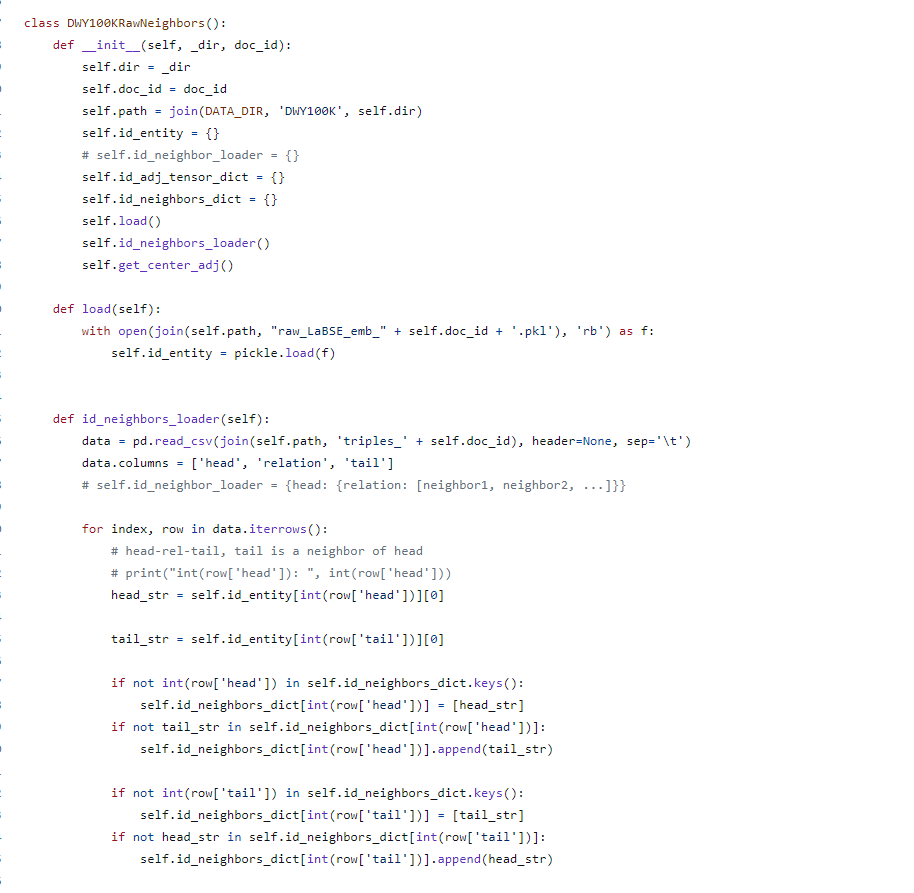
\includegraphics[width=1\linewidth]{figure/loader.png}
    \caption{Process of DWY100K}
    \label{100}
\end{figure}
\begin{figure}
    \centering
    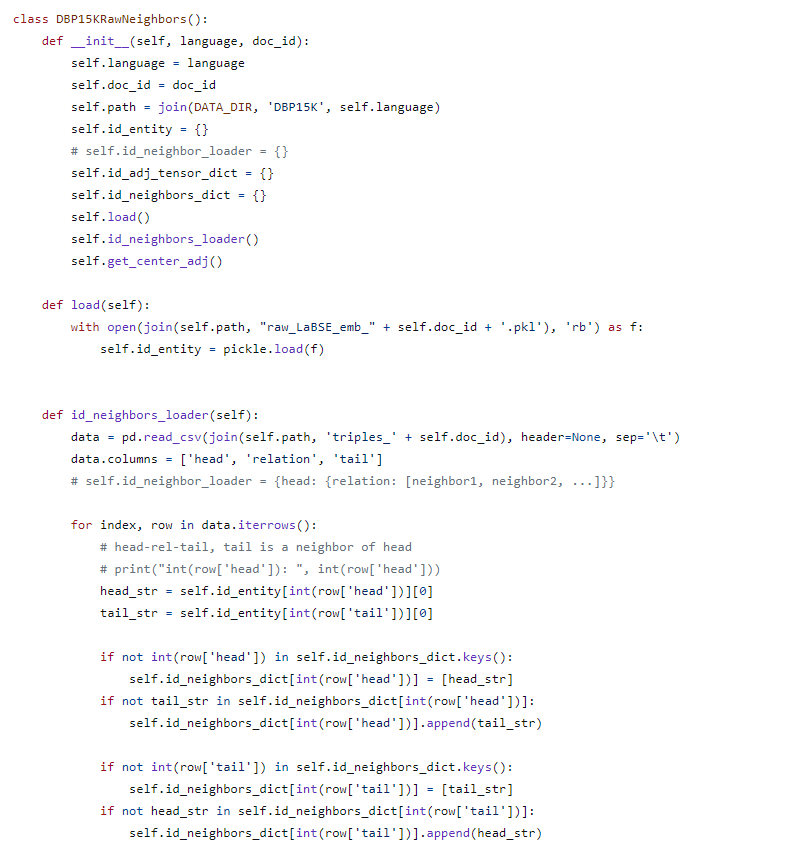
\includegraphics[width=1\linewidth]{figure/loader15k.png}
    \caption{Process of DBP15K}
    \label{15k}
\end{figure}

\end{document}
\endinput
%%
%% End of file `sample-xelatex.tex'.
